\documentclass[11pt,a4paper]{article}

\usepackage[german]{babel} % deutsch, deutsche Rechtschreibung
\usepackage[english]{}
\usepackage[utf8]{inputenc} % Unicode Text 
\usepackage[T1]{fontenc} % Umlaute und deutsches Trennen
\usepackage{mathptmx} % Times New Roman, gewohnter Font
\usepackage{courier} % Schreibmaschinenfont schicker
\usepackage[scaled=.95]{helvet} % was serifenloses wenn gebraucht
\usepackage{graphicx}

\usepackage{listings} 
\usepackage{color}

\definecolor{dkgreen}{rgb}{0,0.6,0}
\definecolor{gray}{rgb}{0.5,0.5,0.5}
\definecolor{mauve}{rgb}{0.58,0,0.82}

\lstset{frame=tb,
  language=Php,
  showstringspaces=false,
  columns=flexible,
  basicstyle={\small\ttfamily},
  numberstyle=\tiny\color{gray},
  keywordstyle=\color{blue},
  commentstyle=\color{dkgreen},
  stringstyle=\color{mauve},
  breaklines=true,
  breakatwhitespace=true,
  tabsize=3
}

\usepackage{float}
\newfloat{listing}{htbp}{scl}[section]
\floatname{listing}{Listing}

\usepackage[paper=a4paper,width=14cm,left=35mm,height=22cm]{geometry}
\usepackage{setspace}
\linespread{1.10} % nicht ganz anderthalbzeilig, nur ein bisschen mehr Platz
\setlength{\parskip}{0.5em} % kleiner Paragraphenabstand
\setlength{\parindent}{0em} 

% Seitenmarkierungen 
\usepackage{fancyhdr} % Schickere Header und Footer
\pagestyle{fancy}
\newcommand{\phv}{\fontfamily{phv}\fontseries{m}\fontsize{9}{11}\selectfont}
\fancyhead[L]{\phv Praktikumsbericht} 
\fancyhead[R]{\phv \thepage}
\fancyfoot[L]{\phv Michael Sandritter}
\fancyfoot[C]{\ } % keine Seitenzahl unten
\fancyfoot[R]{\phv Matrikelnr.: 969663}

% Ein spezielles Paket zum Aufteilen des Literaturverzeichnisses
\usepackage{bibtopic}
\makeatletter
\def\@seccntformat#1{%
  \expandafter\ifx\csname c@#1\endcsname\c@section\else
  \csname the#1\endcsname\quad
  \fi}
\makeatother

\title{Praktikumsbericht}
\author{Michael Sandritter \\ Matrikelnr.: 969663}

\date{\today}

\begin{document}
\maketitle % erzeugt den Titel mit Autor und Datum

\begin{figure} 
    \subfigure{
\includegraphics[width=\textwidth]{images/footer.png}}
%    \subfigure{\includegraphics[width=0.40\textwidth]{images/logo_hsrm.png}} 
%    \subfigure{\includegraphics[width=0.39\textwidth]{images/AOE-Logo_main_v-claim_72dpi.jpg}} 
\end{figure}

\newpage % neue Seite, muss bei einem Artikel eigentlich nicht sein

\section{Praktikumsbetrieb} \label{sec:betrieb} 

Mein Praktikum habe ich bei der AOE GmbH in Wiesbaden absolviert.
Die AOE GmbH hat ihren Hauptsitz in Wiesbaden und ist Dienstleister für Open Source Enterprise Lösungen.
AOE wurde 1999 unter dem Firmennamen AOE media gegründet und agierte anfänglich als TYPO3 Dienstleister.
Inzwischen umfassen die Serviceleistungen Open Source Web Portale, E-Commerce und mobile Anwendungen,
die für globale agierende Unternehmen entwickelt werden.
Das Kollegium umfasst 200\texttt{+} Entwickler und Consultants an 8 globalen Standorten, davon 150 Mitarbeiter in der Zentrale in Wiesbaden.
Die Unternehmenskultur setzt auf die Kernelemente: Open Source, objektorientierte Programmierung und Methoden
wie Agile Software-Entwicklung und Test-Driven-Development. 
Dabei pflegt die AOE GmbH eine dezentrale Unternehmensstruktur. Jedem Kunden wird ein Team aus Entwicklern zur Seite gestellt.
Dieses Team arbeitete von nun an komplett selbstständig und setzt alle Projektphasen in engem Kontakt mit dem Kunden um.


\section{Arbeitsumfeld} \label{sec:umfeld}

Während meines Praktikums war ich als PHP Backend-Entwickler im Congstar-Team tätig.
Das Team besteht aus 20 Entwicklern und acht Testern, die sich ihrerseits wiederum in 4 Sub-Teams aufteilen.
Die Frontend bzw. Backend-Kompetenzen sind dabei gleichmäßig auf die verschiedenen Teams verteilt, so dass jedes Team für sich in der Lage ist, sowohl Backend- als auch Frontend-Tasks zu übernehmen.

Jedes Team arbeitet nach der agilen Softwareentwicklungsmethodik Scrum.
In täglichen “Daily Meetings“ tauschen sich die Entwickler in ihren kleinen Teams über den aktuellen Entwicklungsstand aus, indem jeder Entwickler und Tester, dem Team berichtet, woran er gerade arbeitet und gegebenenfalls schildert welche Probleme bei der Umsetzung existieren.
Zusätzlich finden zwei mal wöchentlich “Weekly Meetings“ statt, bei denen alle Entwickler und Tester zu einem übergreifenden Update des Entwicklungsstand zusammenkommen.
In der großen Runde werden Themen besprochen, die das komplette Team betreffen.
Dazu gehört zum Beispiel, die Einführung und Verwendung neuer Technologien, die Entwicklung oder Änderung der Software Architektur sowie generelle organisatorische Themen.

Während der täglichen Arbeit wird jedes Team von einem IT Analysten (ITA) von Congstar betreut. Dieser hat die Funktion des Scrummasters inne und moderiert beispielsweise “Dailys“ und Sprint Retrospektiven (dazu später mehr). Außerdem ist dieser die Schnittstelle zwischen dem Kunden und dem Team. Somit ist er Ansprechpartner für das Team bei Problemen oder fehlenden Informationen. Er kennt die Abläufe bei Congstar und weiss welcher Ansprechpartner für welches Anliegen der Richtige ist.

Der zeitliche Rahmen gibt vor, dass dem Kunden alle zwei Monate ein neues Softwarepaket mit neuen Features ausgeliefert wird.
Innerhalb dieser Zeit absolviert jedes Team drei Sprints. Die ersten beiden Sprints sind Feature Sprints, welche jeweils eine Arbeitszeit von 3 Wochen umfassen. In diesen beiden Sprints werden neue Stories umgesetzt, welche davor von den Product Ownern (PO) priorisiert worden sind. Das Team entscheidet jedoch für jeden Sprint neu, wie viele Stories realistisch umsetzbar sind. 
Es arbeitet dann zu jeder Story kleinere Tasks aus, die von den Entwicklern geclaimed (Ein Entwicker / Tester “nimmt“ sich eine offene Aufgabe und bearbeitet diese) und umgesetzt werden. Der letzte Sprint innerhalb der zwei Monate ist ein Release Sprint.
Dieser erstreckt sich über die beiden verbleibenden Wochen. Zu dieser Zeit finden Verbundtests statt, bei denen die neu entwickelten Features im Zusammenspiel mit der AAX$^{2}$ getestet werden.


\par
\begingroup
\leftskip=1cm % ggf. verstellen
\noindent Die AAX$^{2}$ ist eine Software aus dem Hause Compax (Compax Software Development GmbH ansässig in Wien, Österreich). Diese ist das Workflow-Management-System von Congstar und beinhaltet unter anderem den Congstar-spezifischen Produktkatalog.
Darin werden alle Congstar Produkte abgebildet, wie zum Beispiel die Post- und Prepaidtarife, mit den dazugehörigen Buchungsoptionen oder die von Congstar angebotenen Endgeräte mit ihren Produktdetails und ihrer Verfügbarkeit.
Die AAX$^{2}$ bietet zur Kommunikation mit externen Anwendungen Soap-Schnittstellen an. Über diese werden z.B.: die Produktdaten durch das AOE System abgerufen.
\par
\endgroup

Im laufe des Release Sprints, besteht für die Entwickler ein Feature-Entwicklungs-Stop, damit das neue Softwarepaket im Verbundtest getestet werden kann.
Anstatt neue Features zu entwickeln, wird die Zeit zum Beispiel zum Refactorn der Software oder zum Updaten von Frameworks genutzt. Alternativ wird neue Software ausprobiert, neue Techniken erlernt und vorhandene getestet oder aufgeräumt.
Falls im Verbundtest Fehler auftreten, werden diese bewertet und falls kritisch behoben.

Am Ende jedes Sprints findet zusammen mit den Stakeholdern (Congstar PO's und ITA's) der Sprintwechsel statt, bei dem das Entwickler-Team die Ergebnisse des aktuell endenden Sprints präsentieren und den nächsten Sprint vorbereitet.
Dafür fahren die Entwickler-Teams nach jedem Feature-Sprint nach Köln zu Congstar und nach Ende des Release-Sprints kommen die PO's und ITA's nach Wiesbaden um den Sprintwechsel bei AOE durchzuführen.
Hauptsächlich geht es um die Präsentation der Stories, die innerhalb des letzten Sprints erfolgreich umgesetzt werden konnten.
Das Entwickler-Team führt in diesem Zug auch eine Retrospektive des vergangenen Sprints durch und berichtet, was während des Sprints gut gelaufen ist, welche technischen Probleme und Hindernisse sich ergeben haben und wie diese Probleme gelöst wurden.
Die Stakeholder haben in diesem Zuge die Möglichkeit offene Fragen mit den Entwicklern direkt zu klären. Alle Beteiligten erhalten somit einen Überblick über den aktuellen Stand des Projekts.
Das Review dient als Grundlage für das darauf folgende Sprint Planning, welches festlegt, was im nächsten Sprint bearbeitet werden soll.
Grundlage des Plannings ist das Produkt-Backlog, dort werden durch die PO's Stories gesammelt, welche künftig umgesetzt werden müssen.
Diese Stories gelangen durch neue Features aber auch Bugs in das Backlog und werden dann von den PO's priorisiert.

Während des Sprint Plannings werden im ersten Teil die Stories im Backlog gegroomt, also abgeschätzt wie aufwändig die Stories sind.
Als Ergebnis des Groomings werden der Story Punkte zugewiesen. Diese dienen dem Vergleich der Stories untereinander und der Abschätzung des gesamten Sprintumfangs. Eigentlich vergleicht man Punkte nicht mit einer Zeit Einheit, jedoch erhält jedes Teammitglied im Laufe des Projekts ein Gefühl dafür wie aufwendig bestimmte Aufgaben sind und wieviel Punkte das Team im Laufe einer Arbeitswoche umsetzen kann. Anfangs waren beispielsweise meine geschätzten Punkte sehr stark abweichend von denen meiner Teammitglieder, jedoch habe ich relativ schnell ein Gefühl für das Punkteschätzen bekommen.
Im zweiten Teil des Plannings werden die nun gegroomten Stories im Backlog durch die PO's nochmals mit den neuen Informationen bezüglich des Aufwands priorisiert. Danach wird durch das Entwicklerteam festgelegt wie viele der besprochenen Stories umgesetzt werden können. Das hier gesetzte Sprintziel sollte erreichbar sein, was die Entwickler durch ihre Aussage versichern.

Falls Stories schneller umgesetzt werden als geplant, kann immer eine Story aus dem Backlog nachgezogen werden. Jedoch sollte dies das Sprintziel nicht beeinflussen. Sollten dennoch ungeplante Ereignisse oder Abhängigkeiten eintreten, welche eine Story verzögern, kann diese überkippen in den nächsten Sprint. Dies sollte jedoch möglichst vermieden werden

Nachdem die Stories für den nächsten Sprint festgelegt sind, definieren die Entwickler für jede Story kleinere Aufgaben (Tasks) und schätzen diese in Minuten, Stunden und Tagen ab. Dabei ist es wichtig, die Aufgaben so klein wie möglich und so groß wie nötig zu wählen.

In unserem Fall werden Backlog, Stories und Tasks im Projekt-Management-Tool Jira verwaltet.

Im Laufe des Sprints werden die einzelnen Tasks von den Entwicklern abgearbeitet.
Zu Beginn einer Aufgabe vermerkt der Entwickler im Jira, dass dieser nun an diesem Task arbeitet, indem er sich den Task claimed, also diesen auf “in Arbeit“ zieht und Jira dann automatisch den Benutzer mit der Aufgabe verknüpft.
Während der Arbeit wird an dem Tasks vermerkt, wie viel Zeit für den Task verbraucht wurde (geburned). Aus der
geschätzten und der letztendlich benötigten Zeit lässt sich ein Burndown-Chart ermitteln, welches den aktuellen Fortschritt des Sprints widerspiegelt.

Sind alle Tasks einer Story umgesetzt steht die Abnahme dieser Story an. Diese erfolgt durch einen Entwickler der an der Umsetzung der Story beteiligt war und durch den Product Owner (PO).
Der Entwickler präsentiert dem PO die Features welche durch die Story umgesetzt werden sollten.
Erfüllt das Umgesetzte alle Akzeptanz-Kriterien, die für die Story definiert wurden, kann die Story durch den PO abgenommen werden und ist somit abgeschlossen.



\section{Projektbeschreibung} \label{sec:projekt}

Mein Team ist zuständig für die Congstar GmbH.

Congstar ist eine Tochterfirma der Deutschen Telekom AG und deutschlandweiter Anbieter für Mobilfunk- und DSL-Produkte.
2008 stellte sich Congstar ein ambitioniertes Ziel: Die komplette IT von Congstar sollte innerhalb eines Jahres ersetzt werden.

AOE hat dabei für Congstar ein komplettes Telco E-Commerce Framework auf Basis des Open Source Content Management Systems (CMS) TYPO3 entwickelt und betreut es seitdem mit aktuell 3 Teams und somit ca. 15 Mitarbeitern allein für den Webbereich.

Congstar vermarktet all seine Produkte vorrangig über das Internet, somit ist das Web nahezu die Kernkompetenz von Congstar. AOE übernimmt dabei die gesamte Web-Entwicklung bestehend aus: Content Management System, Produktkonfiguration und Bestellprozessen, Kampagnen Management System, Kundenservice, Vertriebspartnerportal und White Label-Vertrieb. 

\subsection{Webseiten und Portale}

\begin{figure}[H]
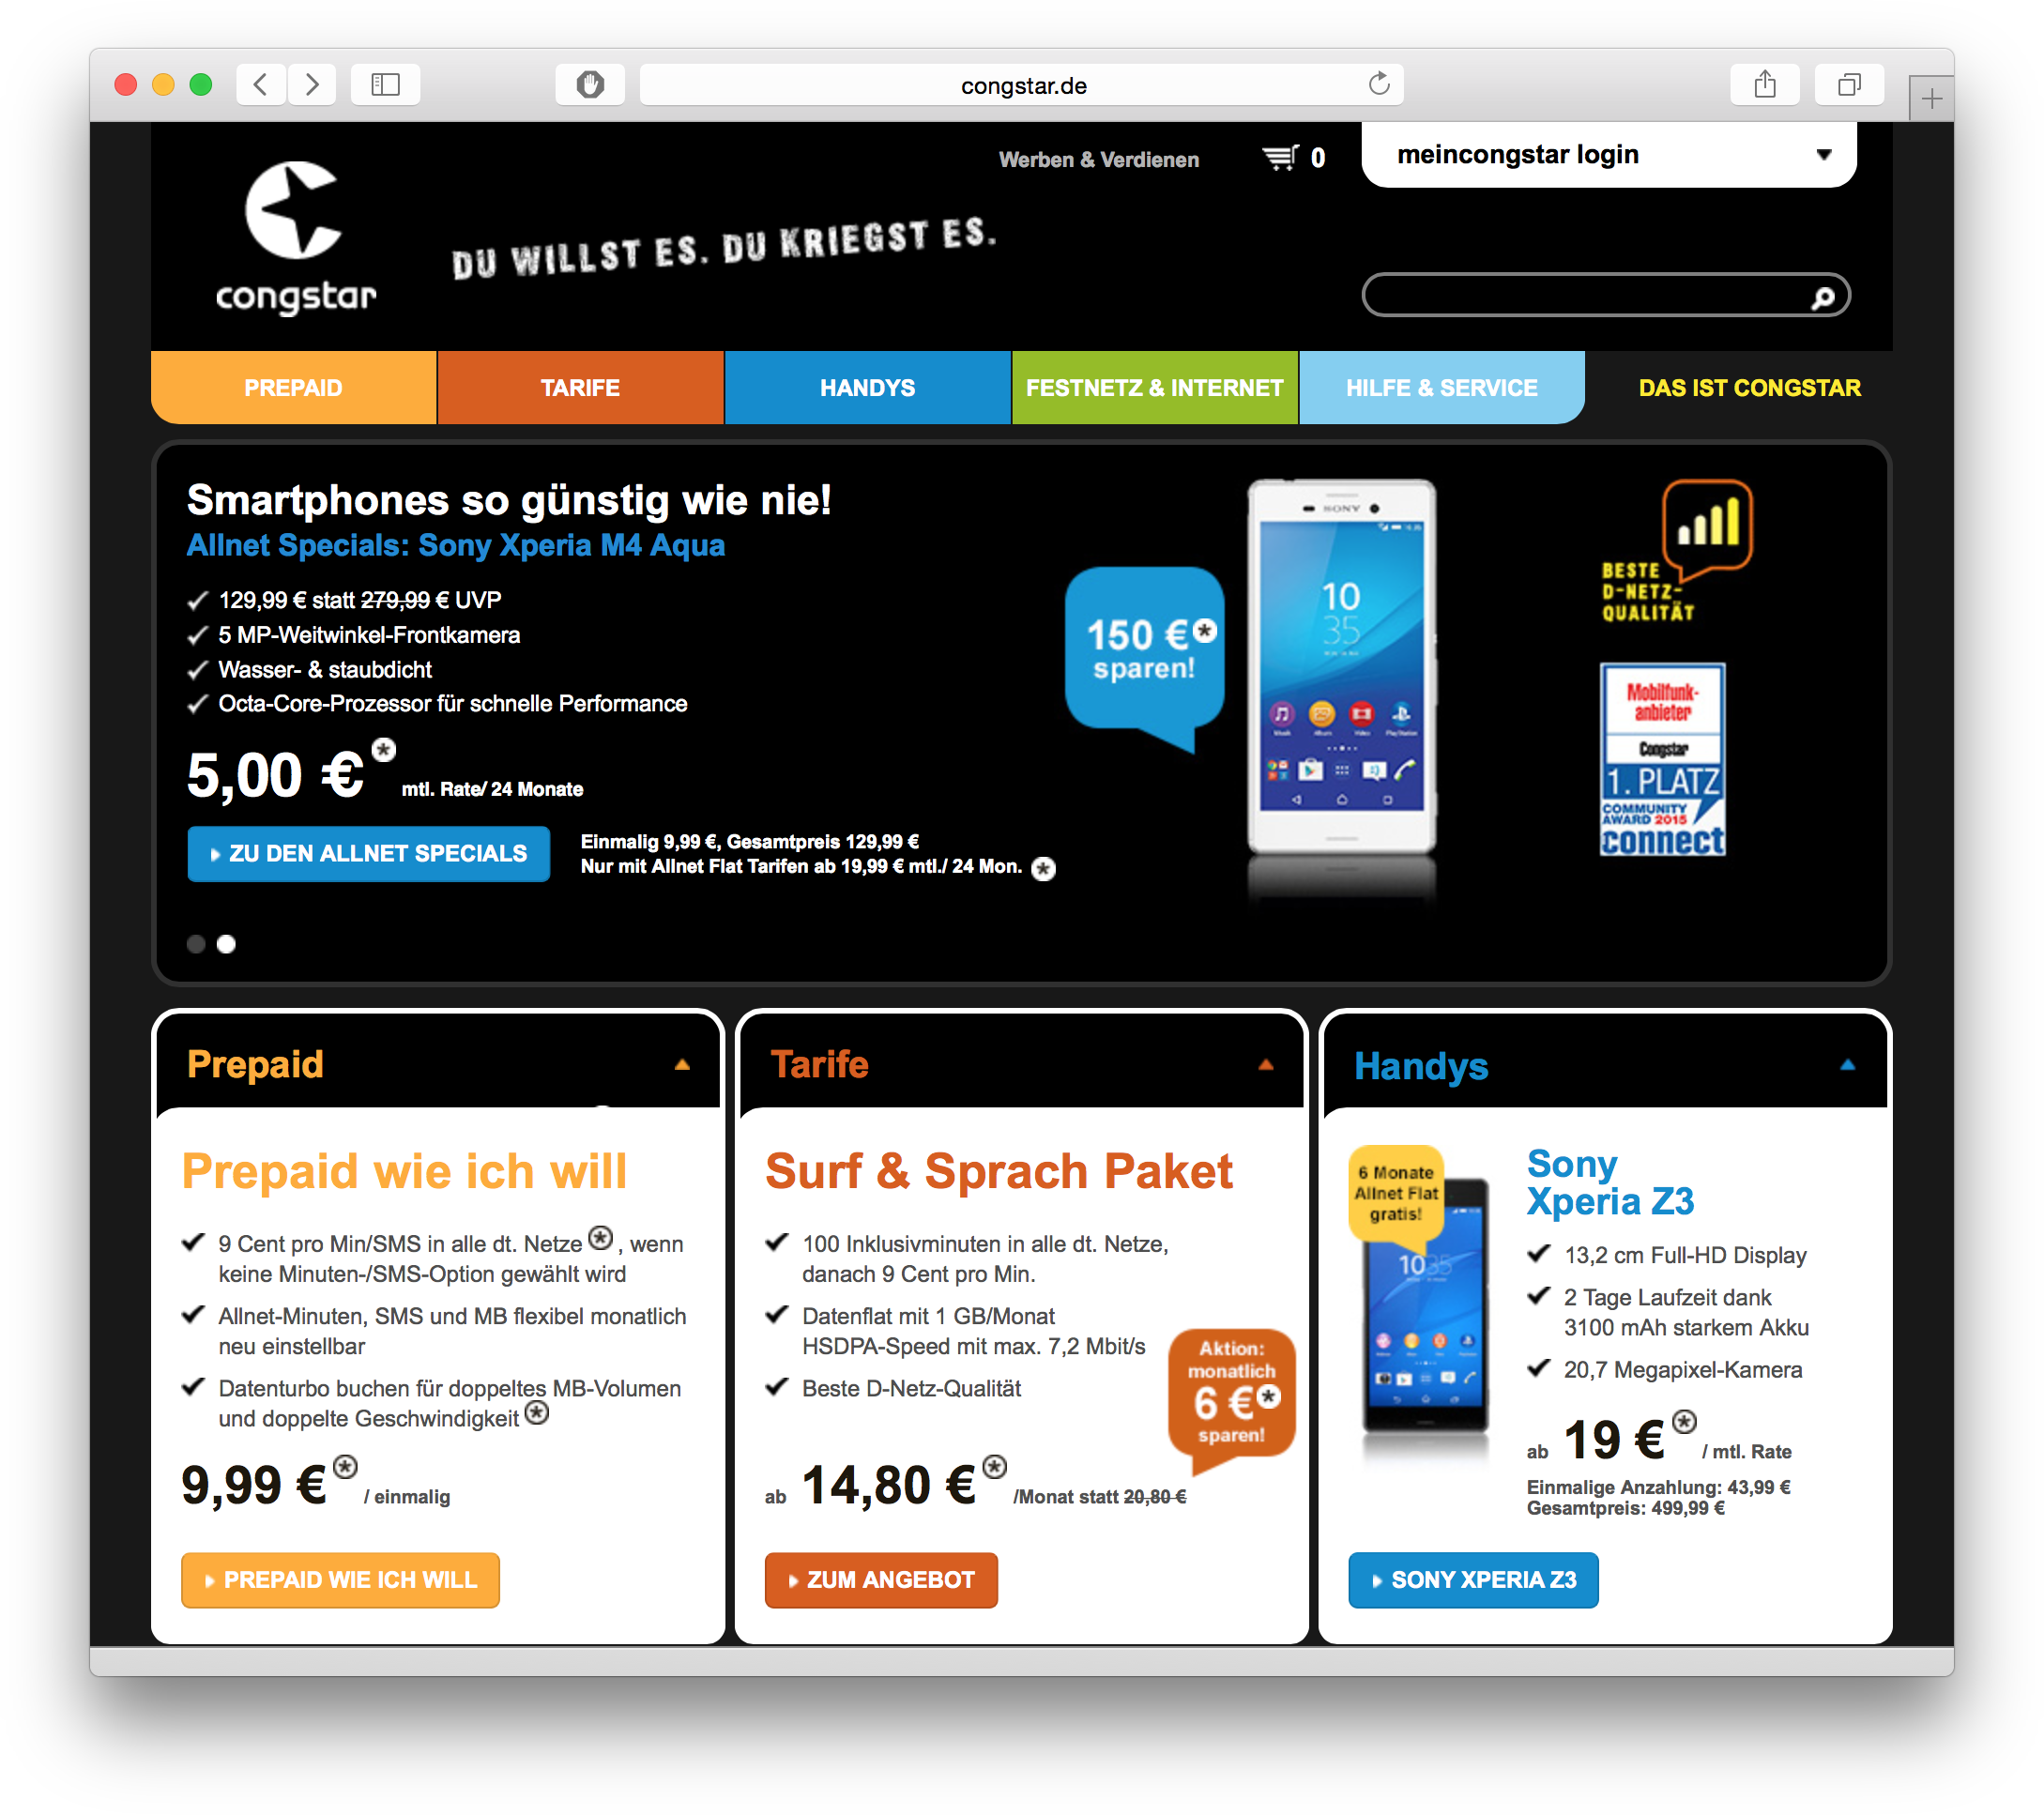
\includegraphics[width=\textwidth]{images/Sites/Congstar_Main.png}
\centering
\caption{Die Congstar Hauptwebseite \cite{congstar}}
\end{figure}

\begin{figure}[H]

\includegraphics[width=0.7\textwidth]{images/Sites/Congstar_Mobil_CSC.png}
\centering
\caption{Das Congstar Mobil Kundenportal (CSC)\cite{congstarcsc}}
\end{figure}

\begin{figure}[H]
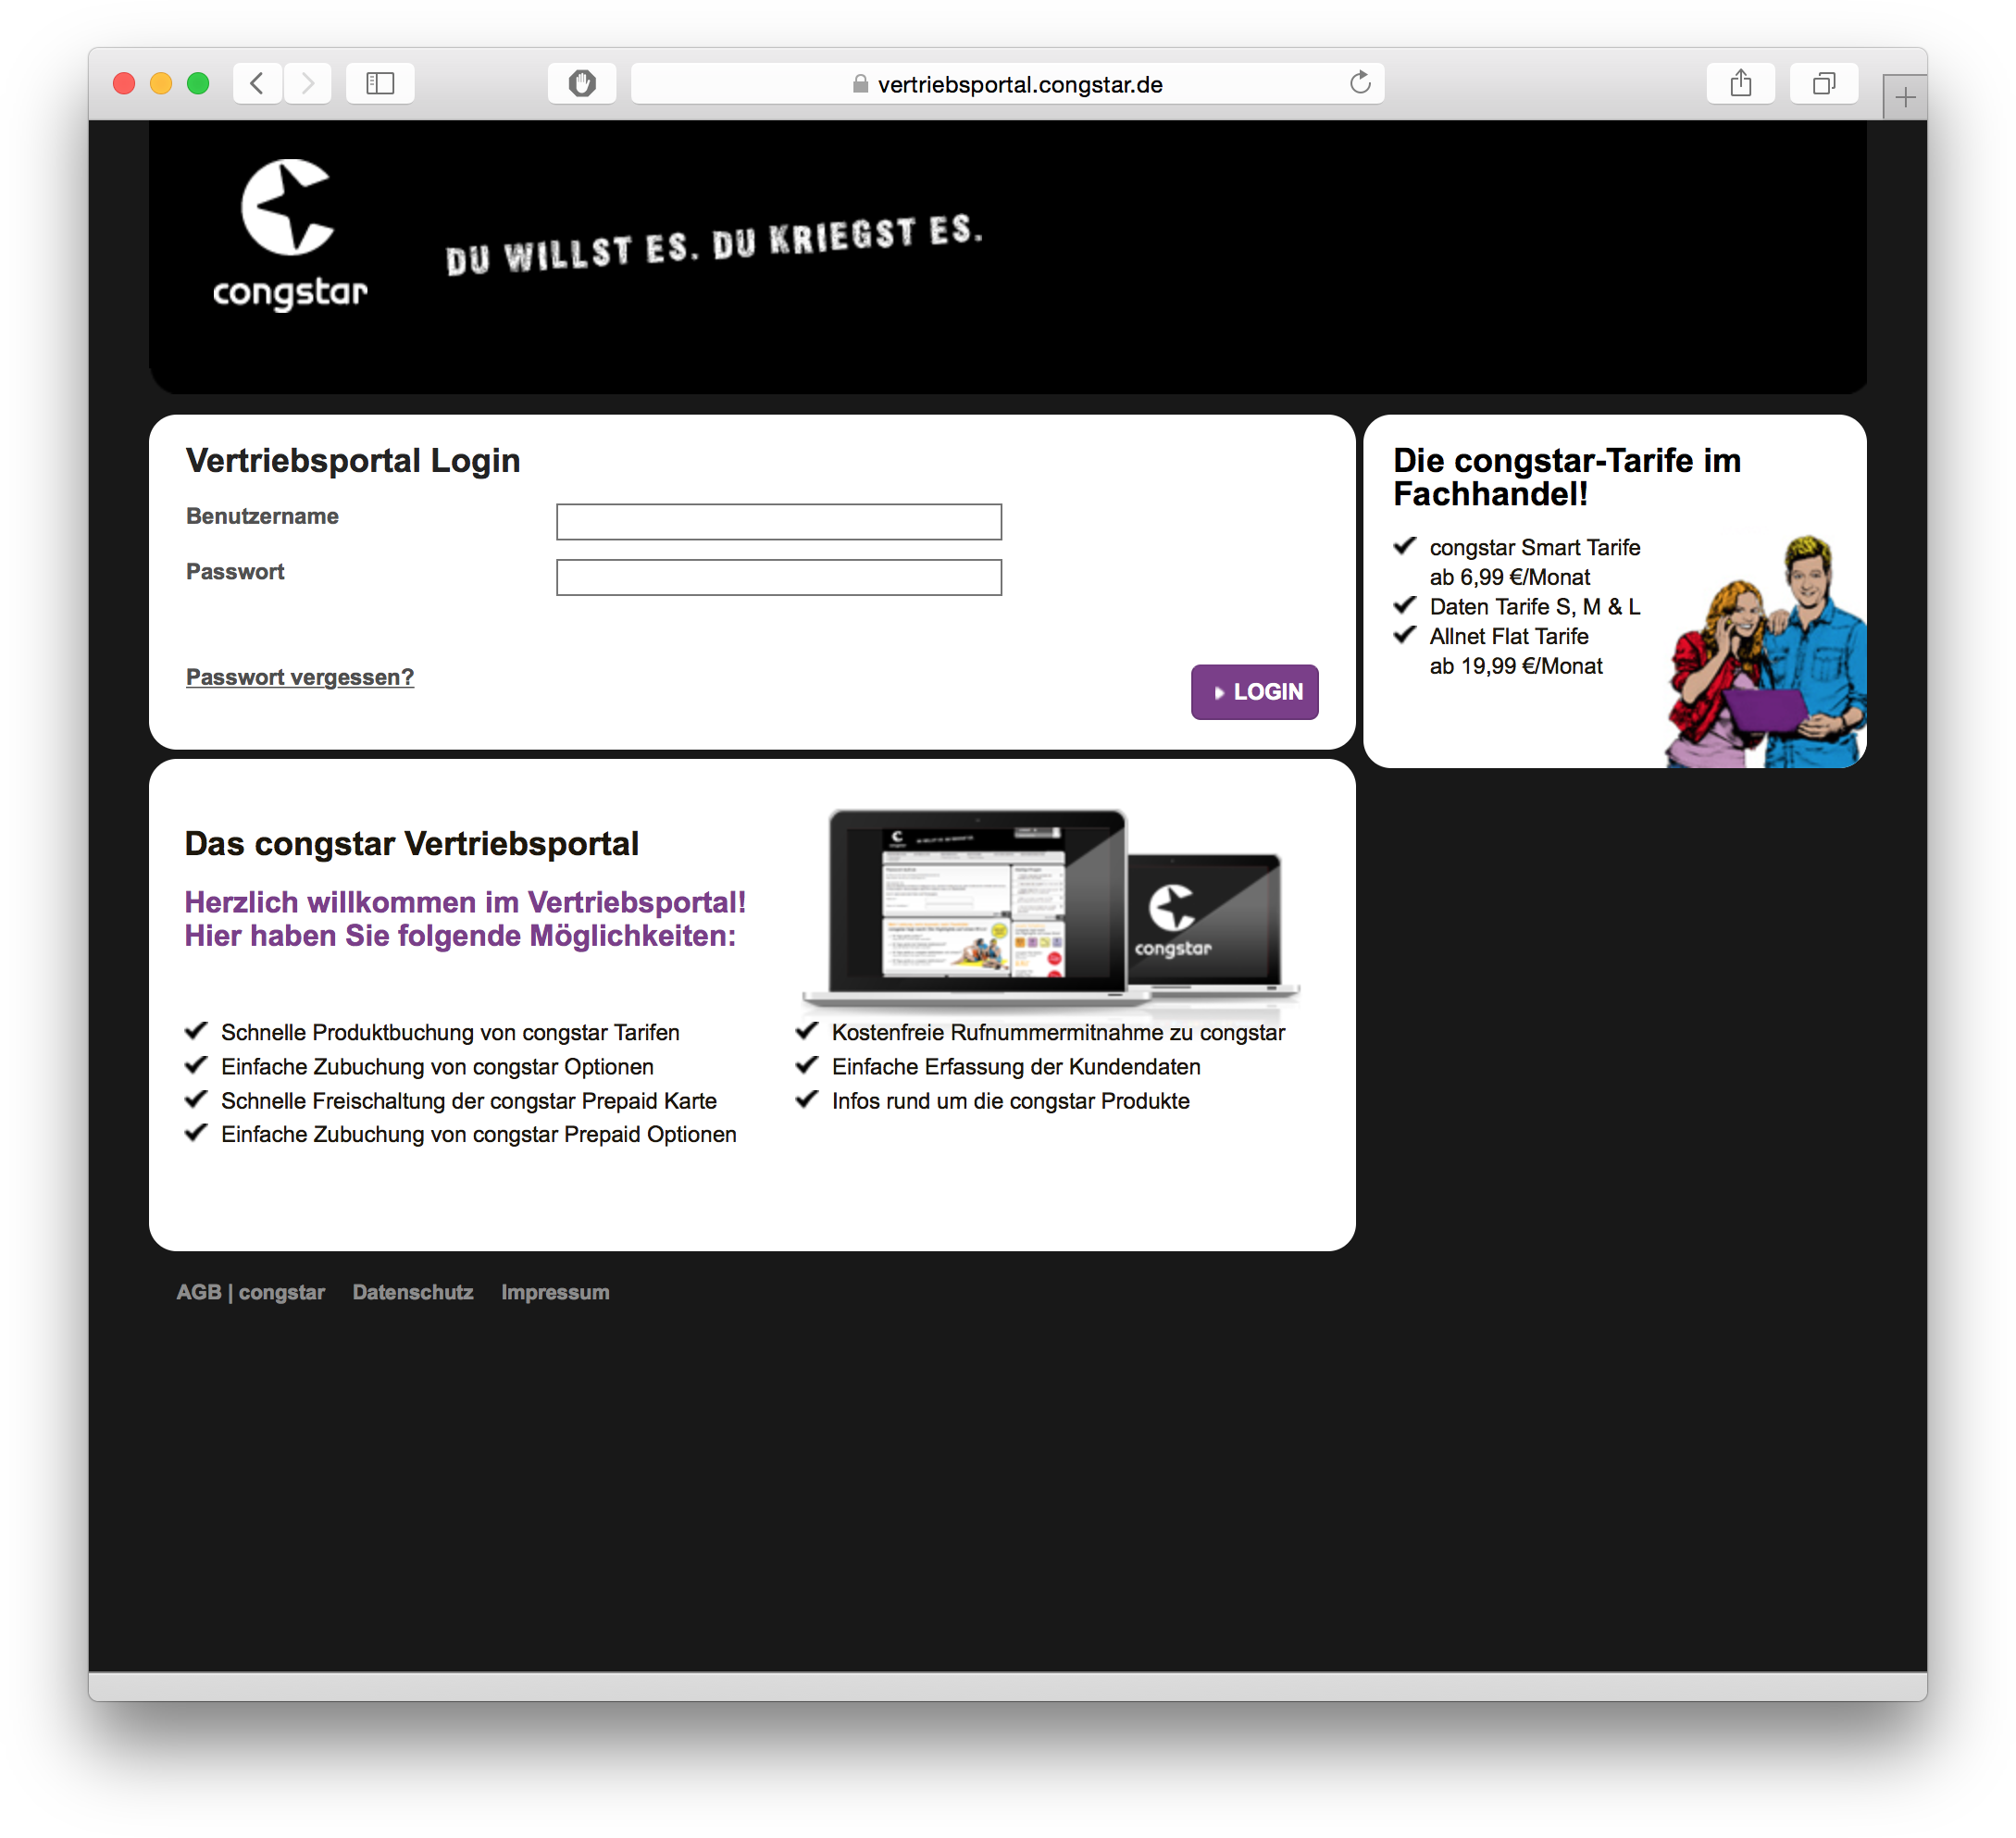
\includegraphics[width=0.7\textwidth]{images/Sites/Congstar_CPP.png}
\centering
\caption{Das Congstar Vertriebsportal (CPP) \cite{congstarv}}
\end{figure}

\pagebreak
Congstar Breitband:

\begin{figure}[H]
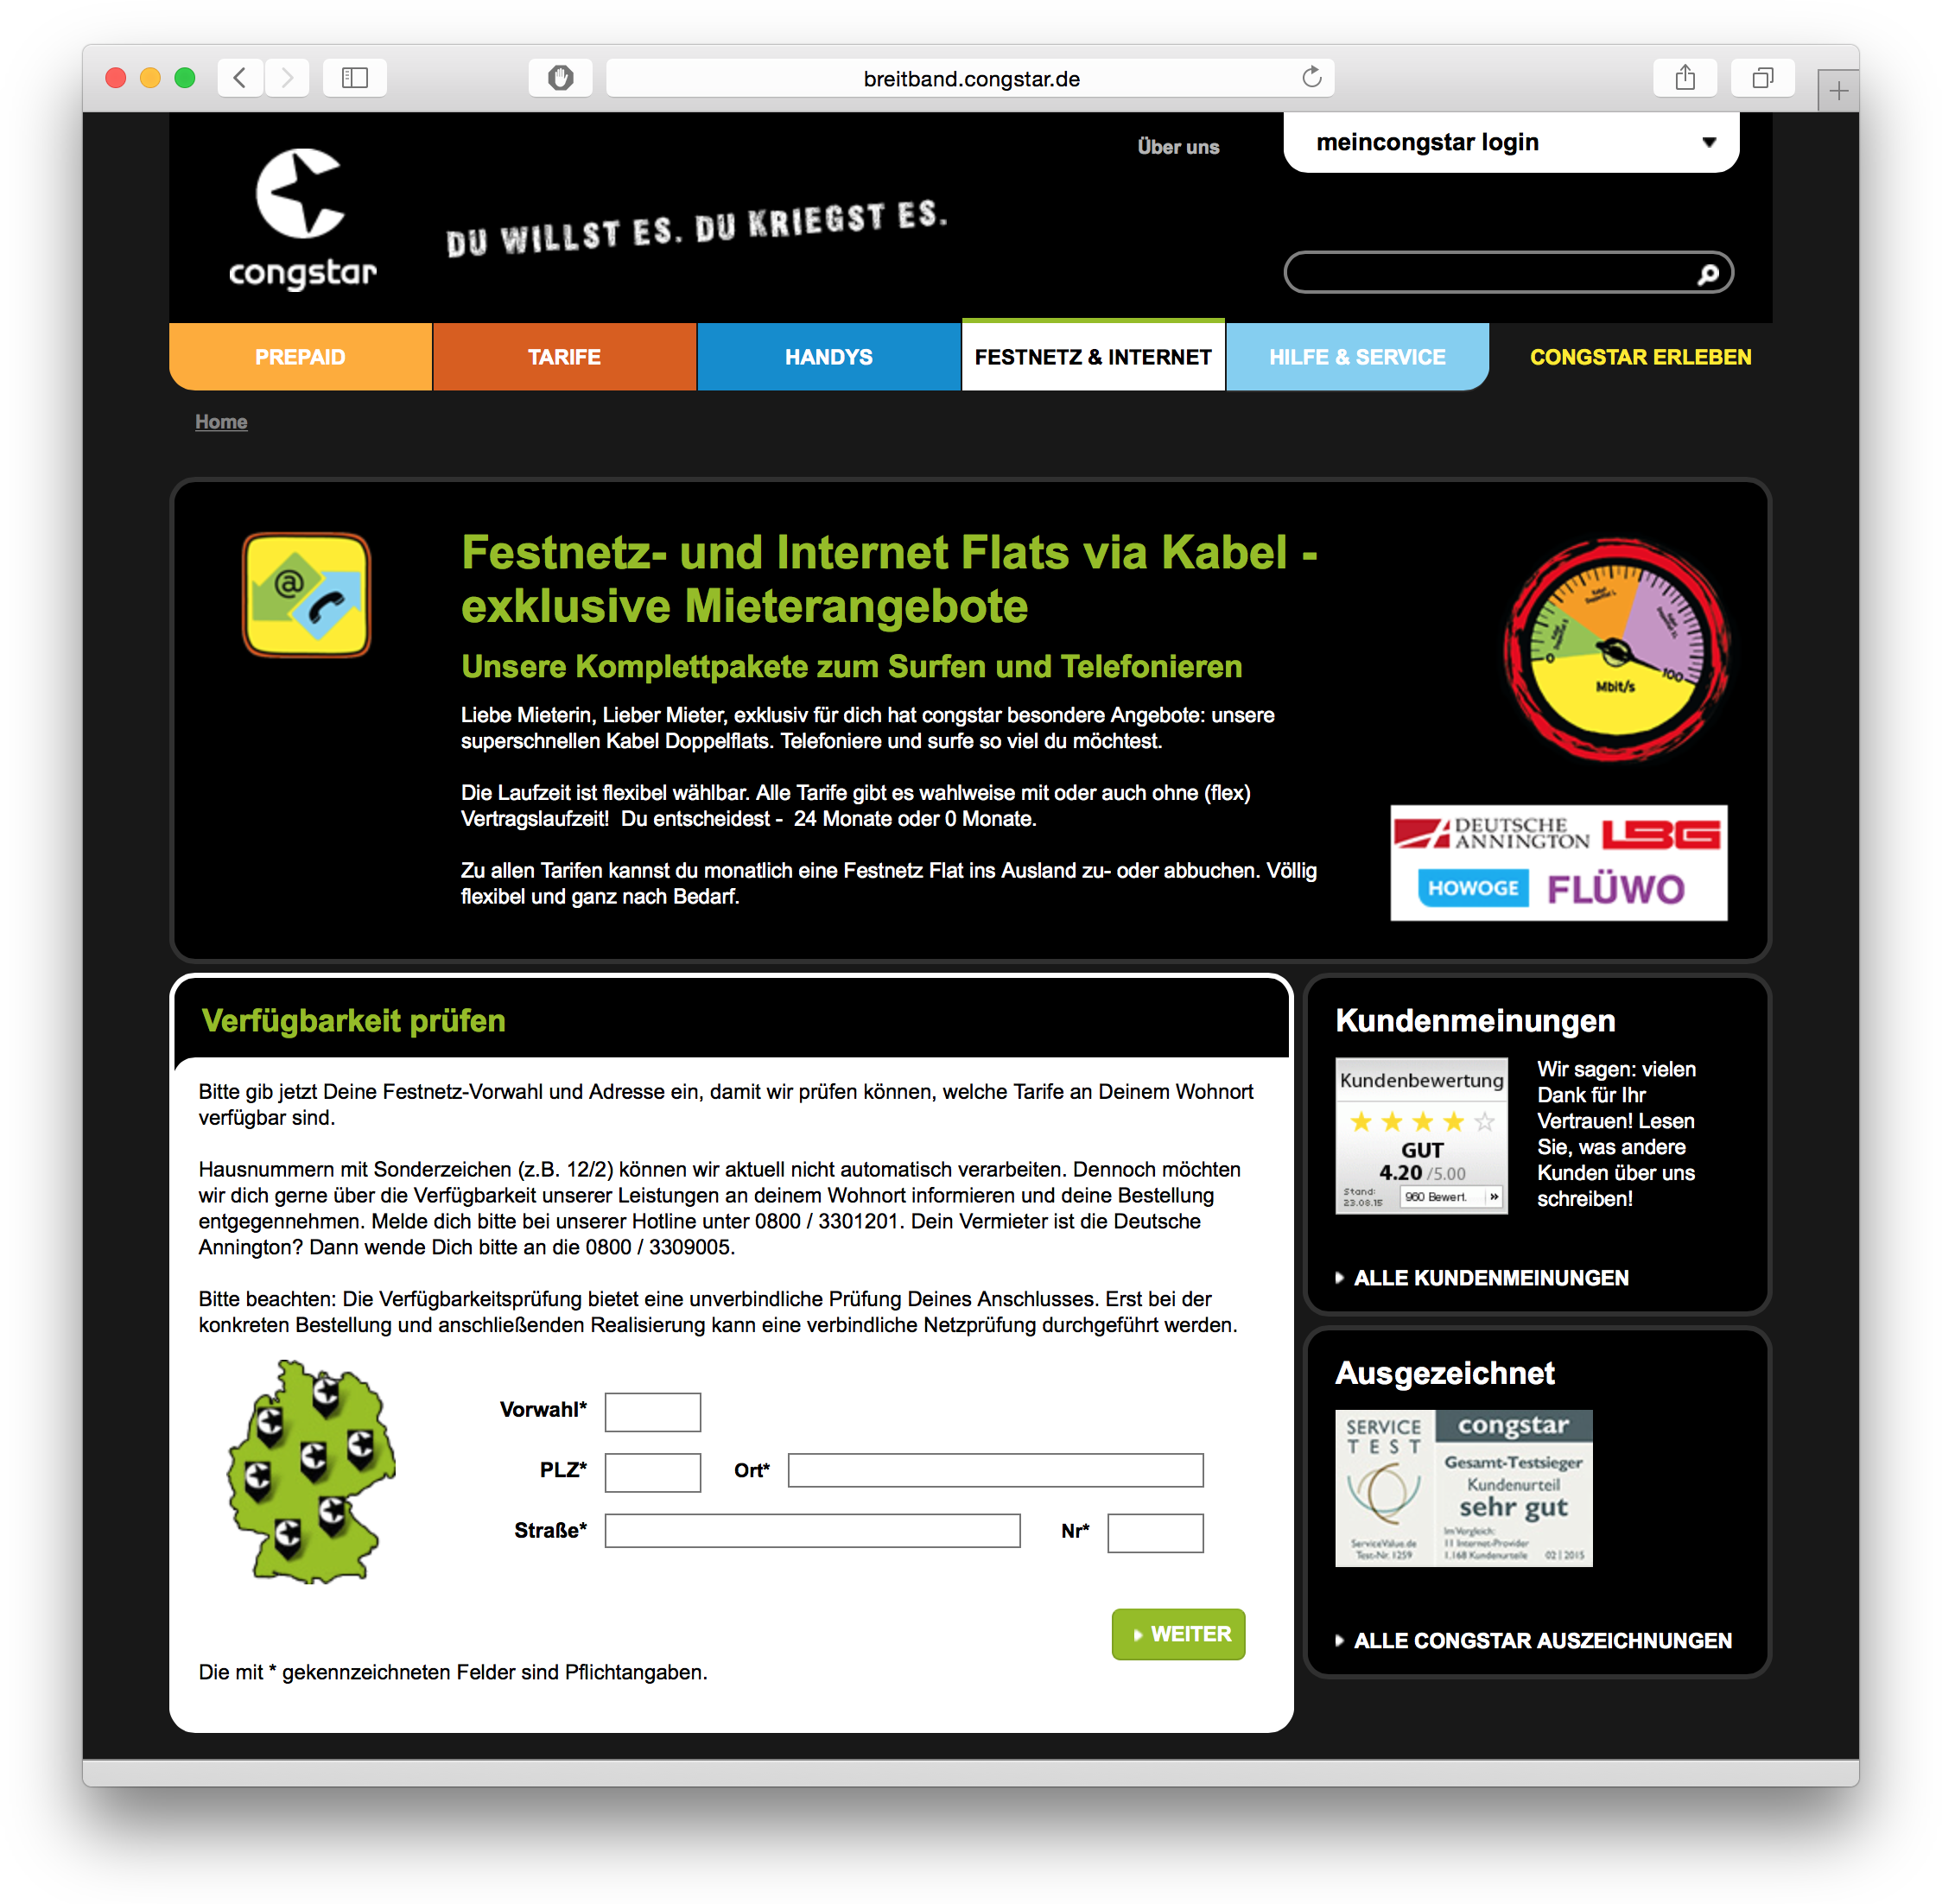
\includegraphics[width=0.7\textwidth]{images/Sites/Congstar_Breitband.png}
\centering
\caption{Die Congstar Breitband Hauptseite \cite{congstarb}}
\label{figure1}
\end{figure}

\begin{figure}[H]
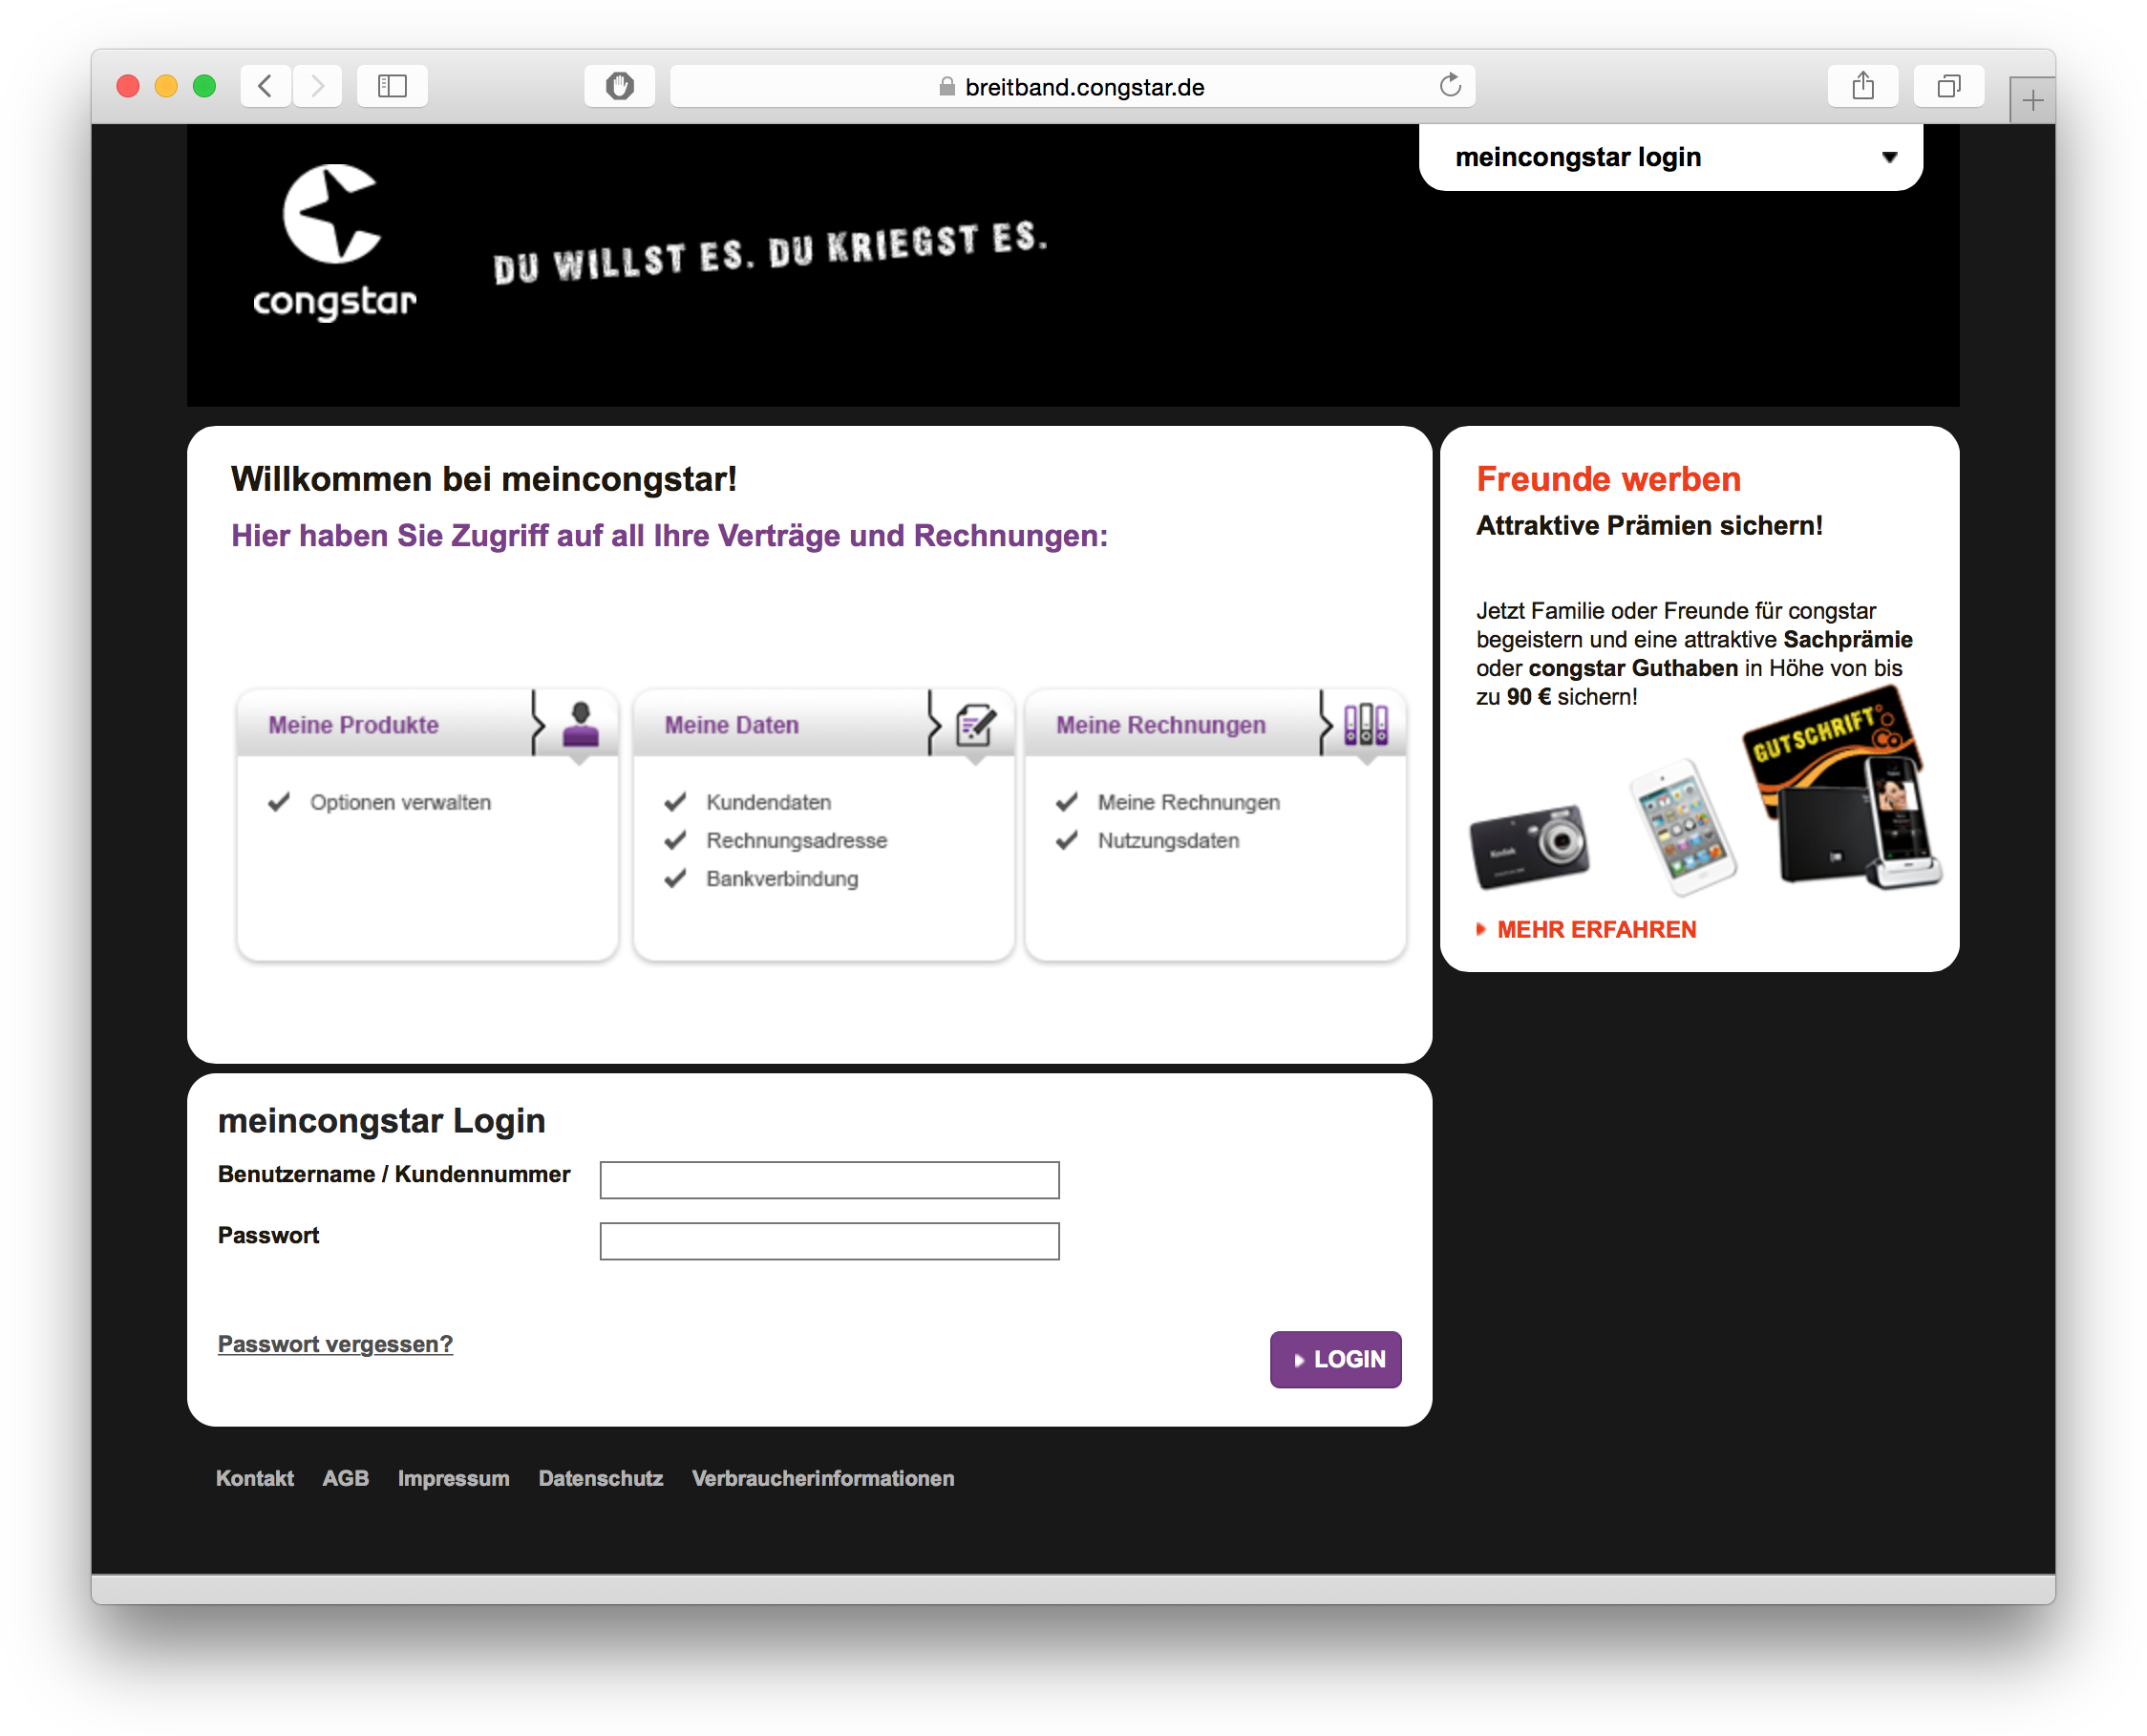
\includegraphics[width=0.7\textwidth]{images/Sites/Congstar_Breitband_CSC.png}
\centering
\caption{Das Congstar Breitband Kundenportal (CSC) \cite{congstarbcsc}}
\end{figure}


\subsection{White Label-Vertrieb}


\begin{figure}[H]

\includegraphics[width=0.7\textwidth]{images/Sites/White_Label/Ja_Mobil.png}
\centering
\caption{Die Ja! Mobil Webseite \cite{ja}}
\end{figure}

\begin{figure}[H]
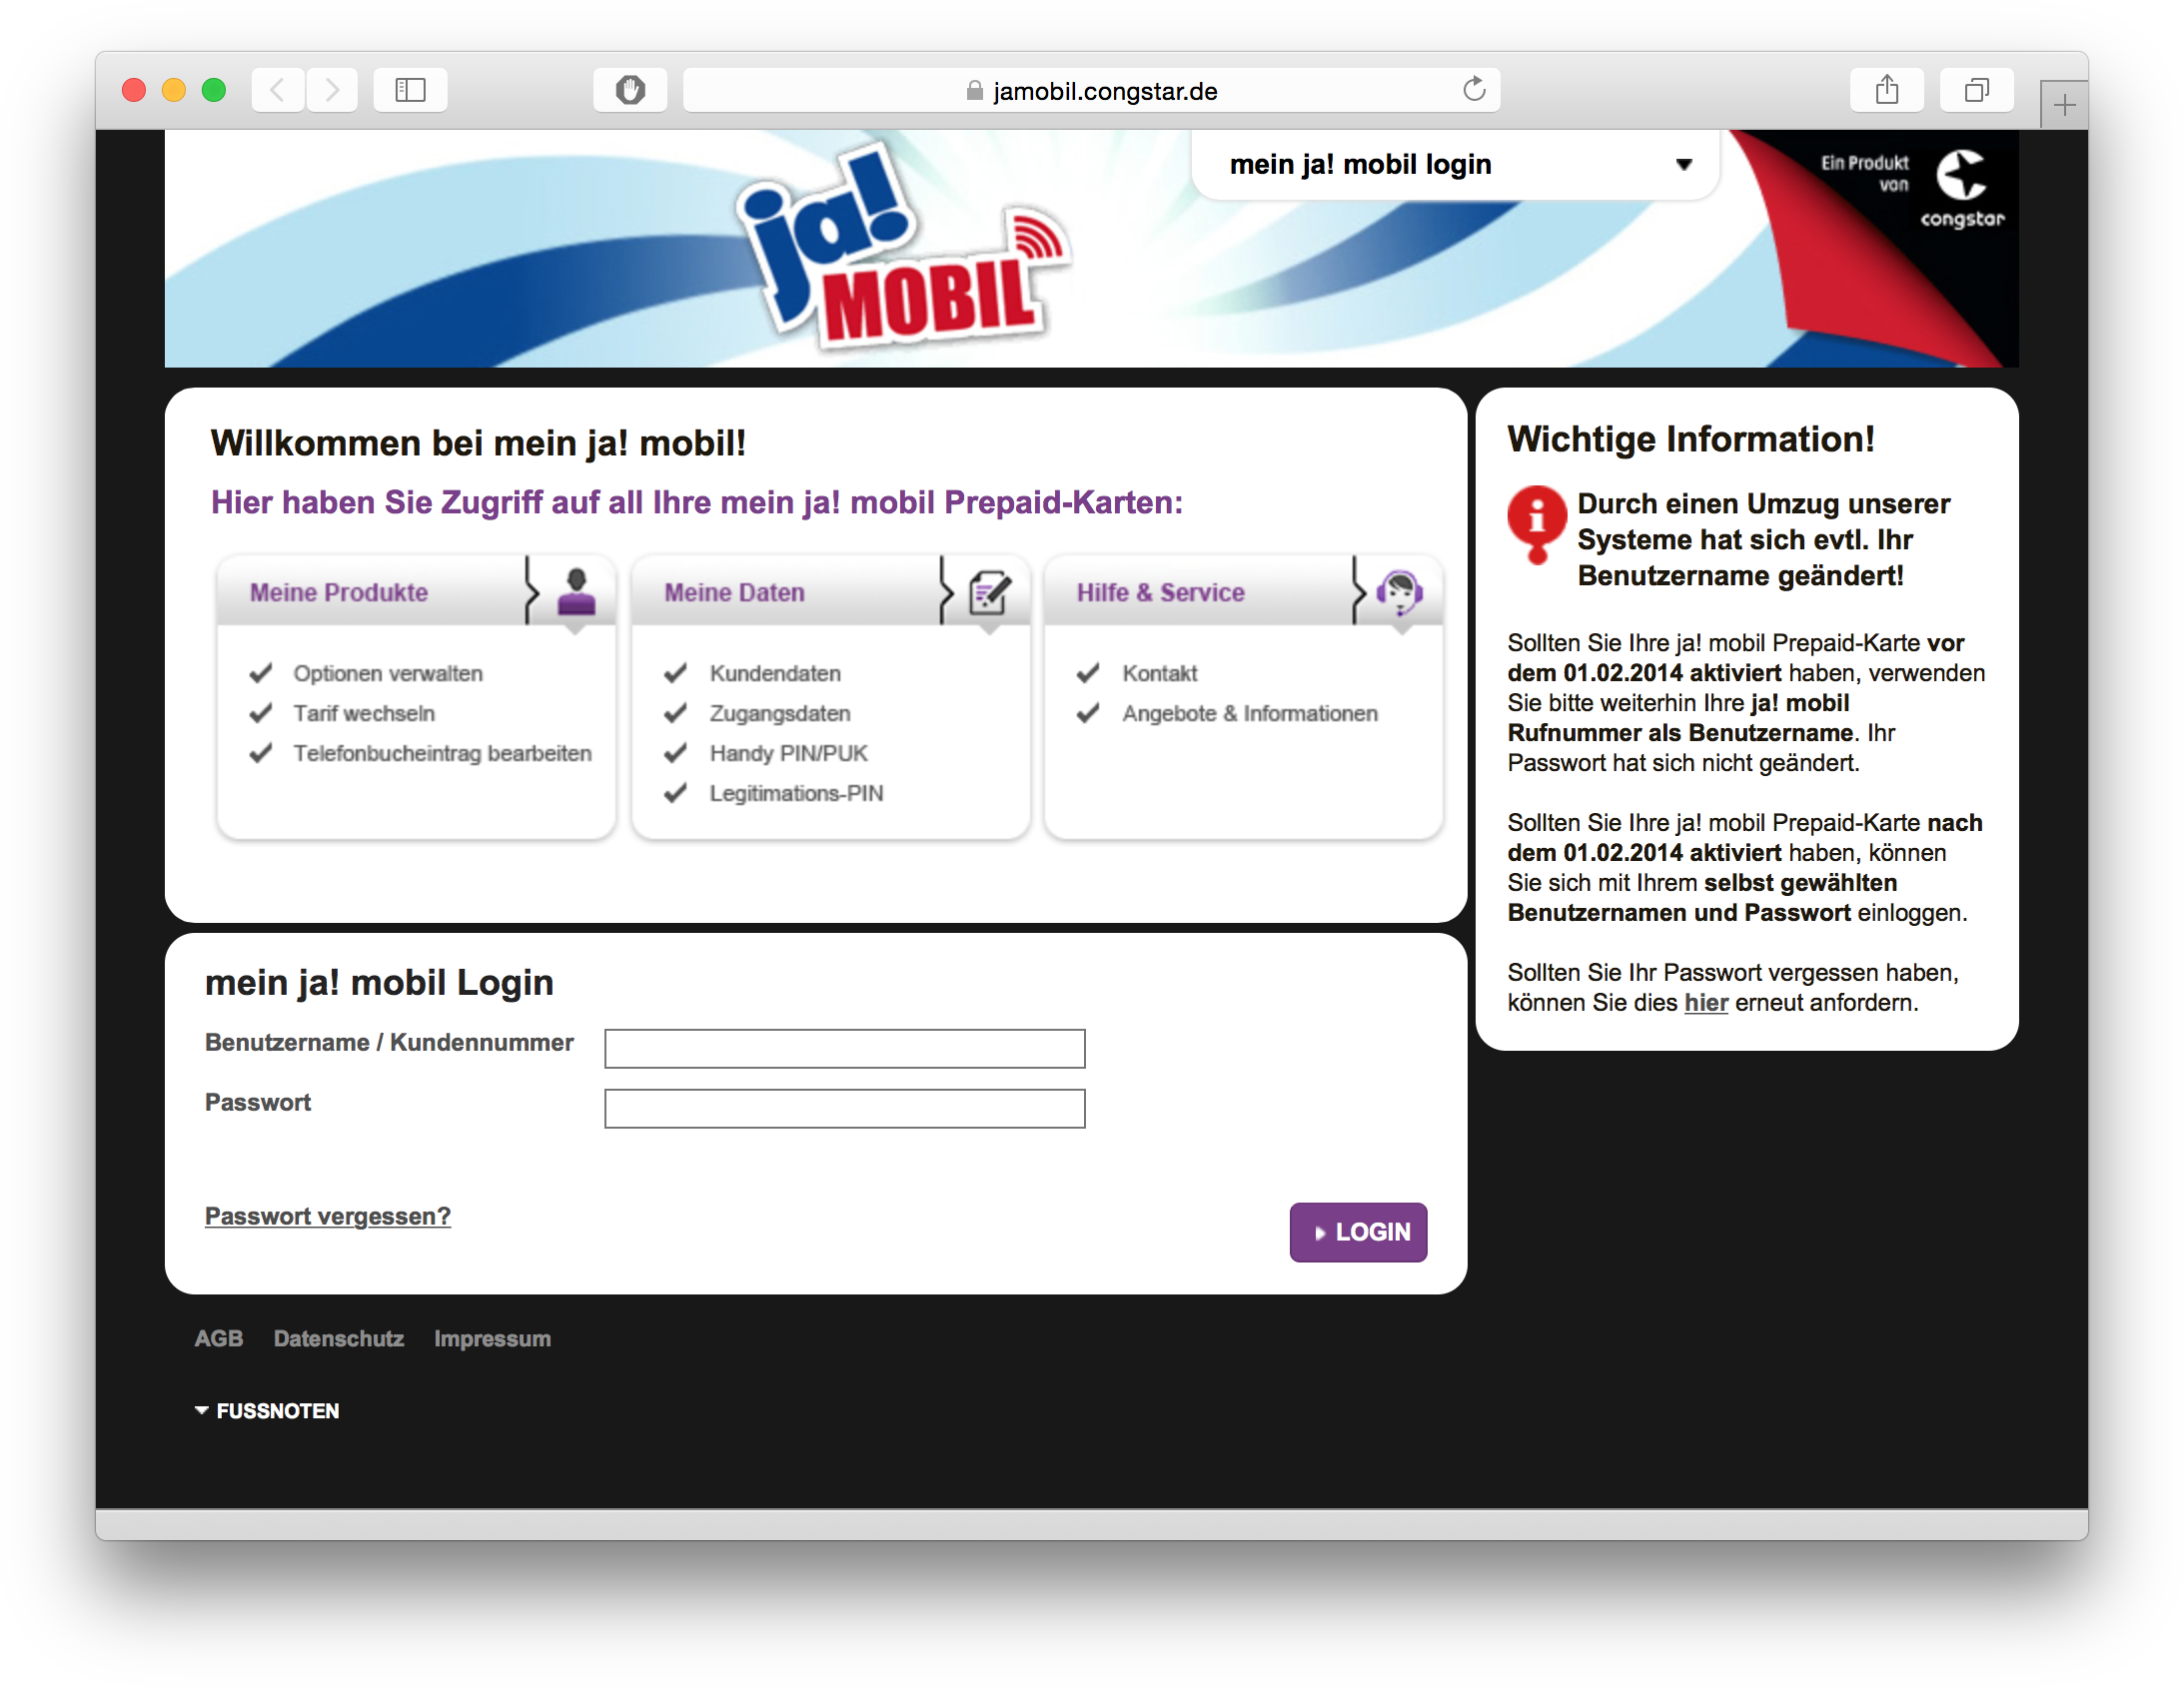
\includegraphics[width=0.7\textwidth]{images/Sites/White_Label/Ja_Mobil_CSC.png}
\centering
\caption{Das Ja! Mobil Kundenportal (CSC) \cite{jacsc}}
\end{figure}


\begin{figure}[H]
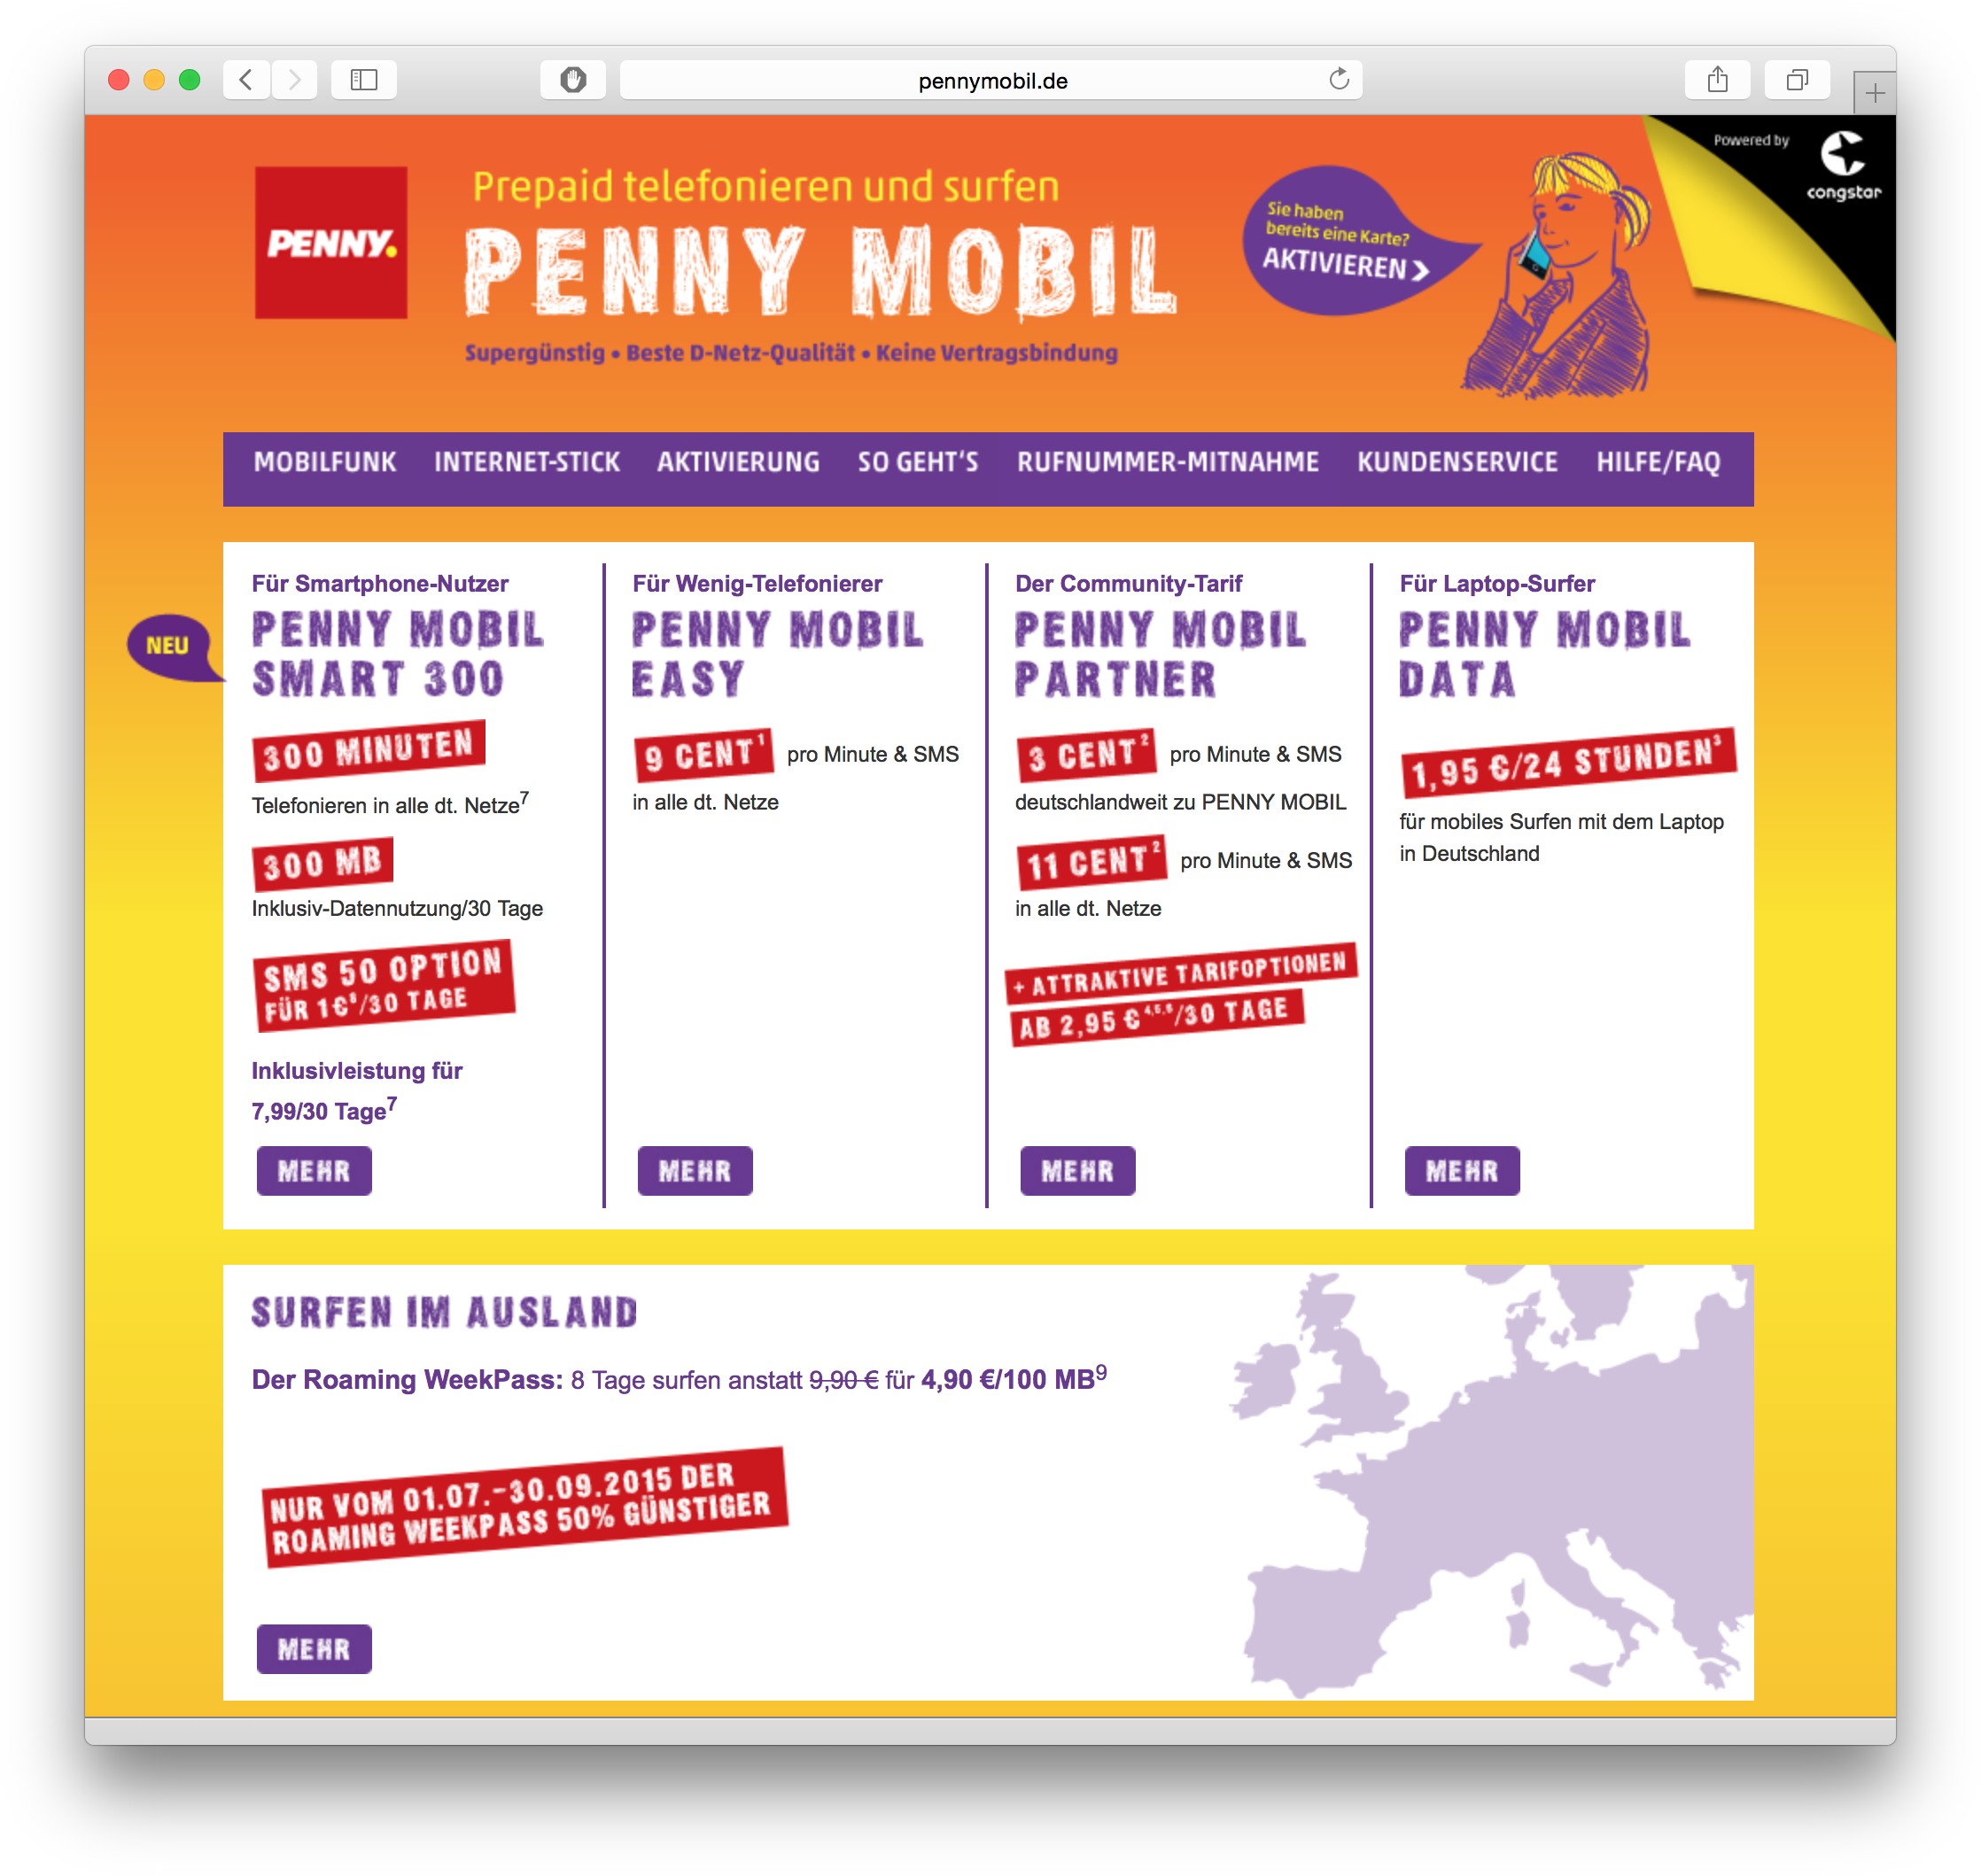
\includegraphics[width=0.7\textwidth]{images/Sites/White_Label/Penny_Mobil.png}
\centering
\caption{Die Penny Mobil Webseite \cite{penny}}
\end{figure}

\begin{figure}[H]
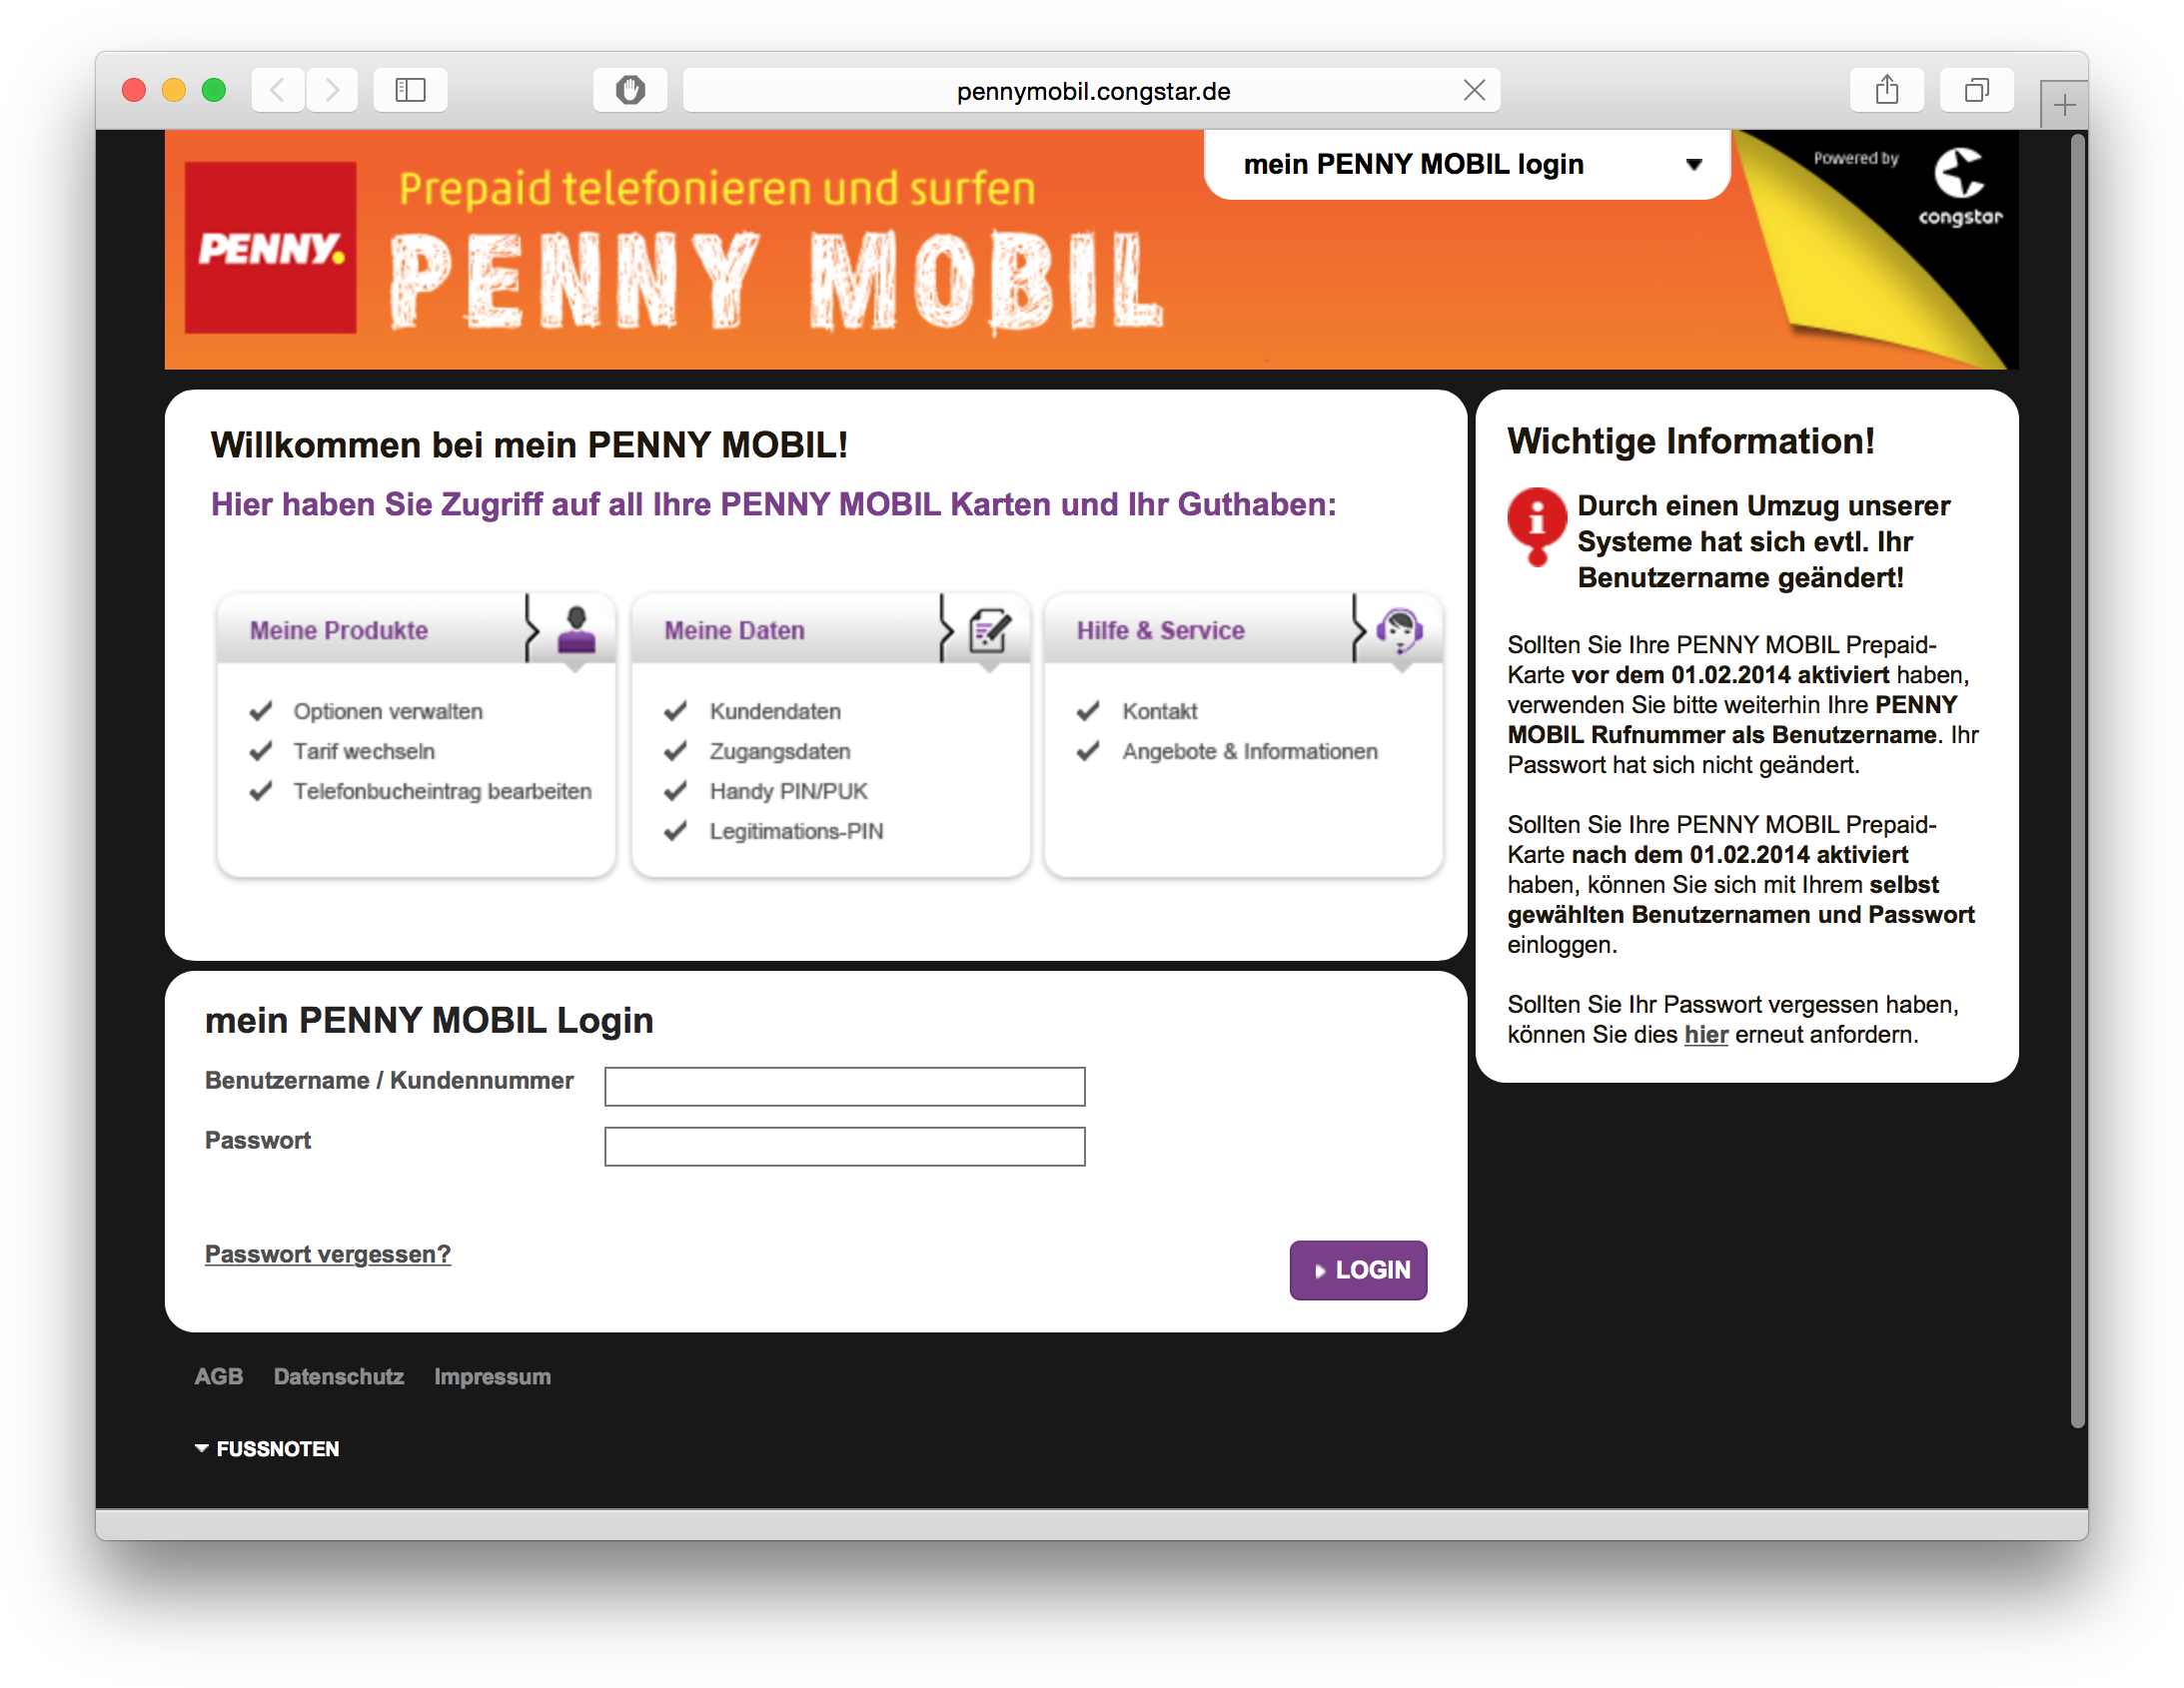
\includegraphics[width=0.7\textwidth]{images/Sites/White_Label/Penny_Mobil_CSC.png}
\centering
\caption{Das Penny Mobil Kundenportal (CSC) \cite{pennycsc}}
\end{figure}


\subsection{Umsetzung}

Die Web-Plattform ist in eine Gesamtarchitektur eingebettet, zu der auch ein zentrales Bestellmanagement- und Workflowsystem sowie ein Billingsystem gehören. Für das Thema Workflow ist die österreichische Firma Compax zuständig, um die Billing-Abwicklung kümmert sich die Firma mr. nexnet.

Eines der Hauptziele war und ist die redundanzfreie Datenpflege und die auf die agilen Geschäftsanforderungen zugeschnittenen Konfigurationsmöglichkeiten. Dies konnte durch die große Anpassungsfähigkeit von TYPO3 realisiert werden.

So können Congstar-Kampagnen und Landing Pages von Marketing- und Sales-Mitarbeitern selbst direkt aus der Plattform heraus erstellt und verwaltet werden. Dadurch gewinnt Congstar sehr viel Zeit. Vorher dauerte es rund sechs Monate, bis ein Produkt auf dem Markt war. Heute kann die so genannte “Time-to-Market“ auf wenige Tage verkürzt werden. In nur fünf Minuten ist eine neue Kampagne konfiguriert und online gestellt.

Ein weiteres Hauptziel des Projekts ist die Content-Personalisierung. TYPO3 ermöglicht Redakteuren Content zielgruppenspezifisch anzulegen: So verändern sich z.B. Preise oder Angebote je nach Einsprung-Link, über welchen die User auf die jeweilige Seite gekommen sind. Selbst auf das individuelle Benutzer-Verhalten, ob Bestandskunde oder Interessent, reagiert das System entsprechend.

Ein weiterer Fokus liegt auf dem Kundenservice: Die Vertragsstrukturen bei Congstar sind flexibel und können vom Kunden modular zusammengestellt und verändert werden. Diese Funktionalität muss ebenfalls online zur Verfügung stehen, da ein Support Mitarbeiter am Telefon oder in einem Geschäft für Congstar hohe Kosten verursachen würde. Deshalb lässt sich das so genannte Customer Self Care (CSC) schnell und einfach durch die Redakteure im TYPO3 anpassen und pflegen.

Die gesamte Lösung “E-Commerce-Framework for Telcos“ oder kurz “EFT“ wurde von AOE speziell für den Einsatz im Bereich Telekommunikation entwickelt und bei Congstar implementiert.

Heute wird das Gesamtsystem von ca. fünf Millionen Besuchern am Tag und Tausend Bestandskunden besucht und genutzt.




\section{Deployment Pipeline} \label{sec:pipeline}

Im folgenden wird der Ablauf der Deployment-Pipeline erläutert.

\begin{figure}[H]
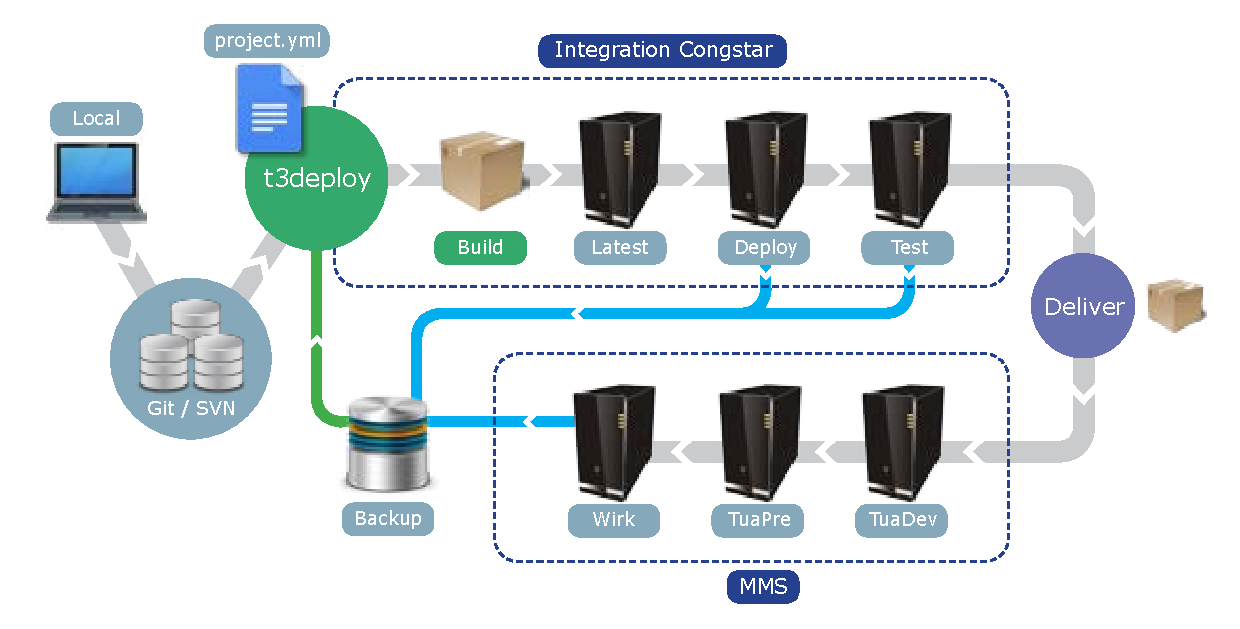
\includegraphics[width=\textwidth]{images/DeploymentPipeline.pdf}
\caption{Der Ablauf der Congstar Deployment-Pipeline}
\centering
\label{fig:pipe}
\end{figure}

Der grobe Ablauf des Deployments (siehe Abbildung \ref{fig:pipe}) besteht darin, dass ein aktuelles Backup aller Systeme, auf welchen relevante Daten gepflegt werden müssen, erstellt und in den Backupstorage geschrieben wird. Dabei werden die Systeme vor einem Deployment gesperrt um zu verhindern, dass die Daten nach dem Backup weiter verändert werden.

Die verschiedenen Systeme unterteilen sich in zwei Hauptgruppen:
\begin{itemize}
  \item Integration Congstar
  \begin{itemize}
    \item wird von AOE gehostet
    \item beinhaltet die internen Deploy-Systeme (VM Ware Server)
    \item Voller Zugriff / volle Verantwortung bei AOE
    \item AOE Teil der Deployment Pipeline
  \end{itemize}
  \item MMS (T-Systems Multimedia Solution)
  \begin{itemize}
    \item wird von der Telekom Tochter MMS gehostet
    \item beinhaltet die externen Deploy-Systeme
    \item (Server Cluster mit verschiedenen Virtuellen Servern)
    \item Kein Einfluss / Zugriff durch AOE
    \item Congstar / MMS Teil der Deployment Pipeline
  \end{itemize}
\end{itemize}

Beim komplett Neubauen eines Softwarepaket, wird zum einen der Quellcode aus den getagten Git-Repositories gezogen und zum anderen die Datenbank und andere Bewegungsdateien aus dem Backupstorage (jeweils von den relevanten Systemen) zusammengeführt.

Die Verheiratung findet mit der Deploymentsoftware T3Deploy statt. Mit Hilfe der Konfigurationsdatei project.yml baut die T3Deploy Software ein fertiges, installierbares Softwarepaket. Die Konfigurationsdatei enthält dabei alle Infomationen über Extensions, Libraries und Datenbanken, die zum Bau eines Pakets notwendig sind.

War der Bau eines Pakets erfolgreich, wird dieses zuerst auf den AOE-internen Umgebungen des Integration Congstar installiert und durchläuft mehrere Teststufen.

Auf der Latest Umgebung werden alle automatisierten Tests durchgeführt. Dazu gehören Unit-Tests, Smoke Tests, sämtliche Code Metriken und Static Cache Tests. Laufen dort alle Tests erfolgreich durch, kann das Paket auf der Deploy Umgebung installiert werden. Dort haben die Redakteure von Congstar die Möglichkeit redaktionelle Änderungen vorzunehmen. Deshalb ist die Deploy Umgebung ein so genannter Content Master. Es werden dort beispielsweise Seiten für neue Features angelegt oder der Inhalt von vorhanden Seiten angepasst. Diese Option ist nötig, da die neuen Features zu dem Zeitpunkt noch nicht auf der Wirk Umgebung (Live System) enthalten sind und somit nur hier angepasst werden können. Ziel der Funktion ist es, dass beim Release direkt eine neue Funktion mit dem passenden redaktionell gepflegten Inhalt online geht. Zusätzlich werden auf dieser Umgebung neue Nutzer für das TYPO3-Backend angelegt, die über das Backupstorage in jedem gebauten Paket zugänglich gemacht werden. Die letzte Umgebung des Integration Congstar bildet die Test Umgebung. Dort laufen hauptsächlich die Java Selenium Tests. Dies sind Tests bei welchen die Seite automatisiert aufgerufen und “durchgeklickt“ wird. Diese Tests prüfen ob alle Workflows “klickbar“ sind und ihr Ziel erreichen.

Sind alle drei AOE-internen Teststufen durchlaufen wird einmal täglich (Nachts) ein fertiges Paket an die MMS geliefert und dort auf der TuADev (Test und Abnahme) Umgebung installiert. Auf der TuADev Umgebung werden Abnahmetests seitens der Congstar Tester durchgeführt, die ebenfalls hauptsächlich Selenium Tests umfassen.

Zu jedem Release wird zuerst die TuAPre Umgebung deployed, da diese dem Wirk System hinsichtlich der Konfiguration am Nähesten ist. Dies wird bereits vor dem eigentlichen Release durchgeführt, um erste Probleme oder Fehler ausschließen zu können.

Das Wirk Deployment wird über Nacht durchgeführt um den laufenden Betrieb möglichst wenig zu stören. Im Wirksystem gibt es sechs Webserver, welche hinter einer Lastverteilung arbeiten. In dieser Umgebung wird ein A/B Deployment oder Schattendeployment durchgeführt. Das heißt, dass einer der Server aus dem Verbund entnommen wird und auf diesem das neue Softwarepaket in ein inaktives Verzeichnis auf dem zentralen Netzwerk Dateisystem (NFS) installiert wird. Dieser Server ist fortan der Schattenserver. Nachdem die Installation erfolgreich durchgeführt und vertestet wurde, wird das “neue“ Verzeichnis wieder inaktiv geschaltet und der Server geht zurück in den Verbund. Nun wird das neue Verzeichnis auf alle Server im Verbund synchronisiert. Sobald alle die neuen Daten erhalten haben, kann in einer sehr schnellen Operation der symbolische Link von dem bisher aktiven Verzeichnis auf das neue umgebogen werden und die neue Software ist online.


\section{Meine Zeit bei AOE } \label{sec:pipeline}

Zu Beginn meines Praktikums stand ich vor einem Berg von “Neuem“.
Neue Techniken in der Webentwicklung,
neue Methoden der Fehlerfindung im vorhanden Projekt und
neue Methoden des Deployments auf den Server
...

Ich lernte sehr viel kennen, wie beispielsweise:

\begin{itemize} 
	\item Debuggen von PHP mit XDebug, 
	\item Arbeit mit virtuellen Vagrant Dev-Boxen, 
	\item Arbeiten mit TYPO3 als CMS, 
	\item Erweitern von TYPO3 mit Extensions und somit dem Nutzen von TYPO3 als Framework, 
	\item Arbeiten im großen Team, 
	\item Organisation der Arbeit im großen Team (Aufgabenverwaltung, Dokumentationsverwaltung, Besprechungen und Abstimmungen), 
	\item Arbeit mit Scrum als Vorgehensmodell, 
	\item Arbeit mit PHPStorm als IDE, 
	\item Anwenden und Einhalten von PHP Code Style Standards, 
	\item Arbeit mit multiplen GIT und SVN Repositories, aus welchen verschiedene öffentliche und private Extensions geladen werden, 
	\item und vieles vieles mehr ...
\end{itemize}



\section{Task 01: Extension zur Reisekostenkalkulation} \label{sec:pipeline}

Da viele Softwaremodule des Congstar Webshop und Vertriebsportal also TYPO3 Extension umgesetzt sind, habe ich im Zuge 
meiner Einarbeitung eine eigene Extension entwickelt, die als Reiseplanungstool eingesetzt werden kann.
Ziel der Extension ist es Personen eine grobe Kalkulation der Kosten offenzulegen, über Reiseziele, 
die sie gerne bereisen würden, von denen sie aber nicht wissen, welche Kosten auf sie zukommen. 
Informationen über Reiseziele und mögliche Kosten sollen über entsprechende APIs angesprochen werden und wurden bei der Umsetzung dieser Extension vernachlässigt.
Der Schwerpunkt der Umsetzung lag in der Erstellung und Konfiguration der Extension, sodass Sie über das
TYPO3 Backend eingebunden werden kann und mit zugewiesener URL im Browser aufrufbar ist.




\section{Task 02: Rollen-basierte Zuordnung der Bestandskundenverwaltung} \label{sec:t02}

Ziel war es, dass die Bestandskundenfunktionalität rollen-basiert zugeordnet werden kann, 
damit sie nur den Sales-Partnern zur Verfügung steht, die die Funktion auch nutzen dürfen.

Dafür wurde im Typo3 Backend eine neue Gruppe für die Bestandskunden-Buchung angelegt.
Redakteure können dadurch die Zuordnung der Rechte im TYPO3 für verschiedene Partner freischalten
oder zusätzlich zuweisen.

Zusätzlich wurde die Funktionalität des Sales-Partner-Objektes erweitert, sodass dieser Auskunft geben kann, 
welche Gruppe er inne hat. Dadurch wird für den jeweiligen Sales-Partner im Congstar Vertriebsportal
nur die Funktionalität zur Verfügung gestellt, die ihm zugeordnet ist.




\section{Task 03: Content Box erstellen und anzeigen}

Damit Kunden bei der POS Kartenaktivierung informiert werden, wie sie den Congstar Mixer bei der POS Kartenaktivierung
nutzen können, soll oberhalb vom Mixer eine Content Box eingeblendet werden, die eine Beschreibung beinhaltet.
Dafür wurde in der eft Extension eine neue Flexform angelegt für die Content Box angelegt.
Diese wurde so konfiguriert, dass die Content Box im TYPO3 Backend von den Redakteuren redaktionell pflegbar ist.
Weiter galt es zu beachten, dass die Content Box zum einen nur angezeigt werden soll,
wenn es sich um ein 9ct. Prepaid Madeira Produkt handelt und zum anderen nur wenn der Mixer angezeigt wird.
Dazu wurde sowohl die Logik im Controller angepasst, als auch das bestehende Template erweitert.




\section{Task 04: Webservice für den Kundenservice implementieren}

Aufgabe war es, die API der eft Extension um die Kunden-Authentifizierung zu erweitern.
Die API der eft Extension ruft dabei über einen Webservice die AAX$^2$ auf, um den Kunden zu authentifizieren.
Dies geschieht über einen SOAP Call 
\begin{lstlisting}
public function authenticateByMtan($customerId, $mTan)
\end{lstlisting}
bei dem eine mTan und die Kundennummer an die AAX$^2$ übergeben wird.
War die Kundenauthentifizierung erfolgreich, so liefert die AAX$^2$ ein Kunden-Objekt zurück, welches
danach in der Session gespeichert wird.
Treten jedoch Fehler auf, sollen folgende Exceptions diese abfangen:

\begin{itemize}
	\item EFT-API wirft Exception A, wenn mTan falsch/ungültig
	\item EFT-API wirft Exception B, wenn mTan abgelaufen (das passiert nach 20 Minuten)
	\item EFT-API wirft Exception C, wenn der Webservice der AAX$^2$ nicht verfügbar ist
\end{itemize}



\section{Task 05: Konfiguration eines Jenkins Job}

\subsection{Schritt 1: build.xml mit Ant ohne Jenkins erstellen}
Zunächst einmal war es Ziel zu verstehen, wie eine build.xml aufgebaut ist
und aus welchen Befehlen sie besteht, um im Nachgang nachvollziehen zu können, auf welchen
Grundlagen die Einstellungen im Jenkins aufbauen.
Um Ant besser kennenzulernen, habe ich mir als Aufgabe gesetzt eine eigene build.xml
zu schreiben, die das Bauen meiner eigenen Reisekalkulations-Extension übernimmt.

Folgende Schritte sollten dabei berücksichtigt werden:

\begin{itemize}
	\item Löschen des Workspace Ordners vor dem Komponenten-Bau
	\item Auschecken der Source Dateien der Komponente aus dem Repository
	\item Laden der Abhängigkeiten über Composer in den Vendor Ordner des Build Workspaces
	\item Verpacken ausgewählter Dateien als ZIP Datei
\end{itemize}

Darüber hinaus habe ich mich mit dem Erstellen eigener Targets beschäftigt und
die Ausführungsreihenfolge mit dem depends Attribut gesteuert.

\subsection{Schritt 2: Build-Job mit Jenkins konfigurieren}

Das Konfigurieren des Build-Jobs in Jenkins ging danach einfach von der Hand.



\section{Task 06: Erstellung von Databuildern}

Im Laufe meines Praktikums wurde die eft-core Extension ins Leben gerufen, die sehr allgemein gesagt,
das Domain Model der eft Extension abstrahiert und dieses den darüber liegenden Schichten zur Verfügung stellt.
Dabei werden in den jeweiligen Unit Tests der eft-core Extension, oft Objekte der eft Extension benötigt.
Wenn man nun in jedem Unit Test, händisch die Mock-Objekte für eft Objekte erzeugen müsste, entstünde viel 
Fleißarbeit. Durch das Verwenden von Databuildern kann dies reduziert werden. Die Databuilder übernehmen dabei das
Generieren der Mockobjekte, sodass die Unit Test schlanker werden.



\section{Task 07: Durchstich OptionsGroups}

Für die neue Madeira Produktreihe wurde ein Rest Endpoint 'getOptions' implementiert,
der bei erfolgreichem Aufruf Optionsdaten zurückliefert.
Der Durchstich durch alle Ebenen erfolgte mit einem schlanken OptionsGroup-Objekt (Walking Skeleton), um 
die grundlegende Funktionalität des Aufrufs zu testen.
Dabei durchlaufen die Daten mehrere Ebenen, in denen, die von der jeweils unteren Schicht kommenden Daten
konvertiert werden, um für die darüber liegende Schicht aufbereitet zu werden.


\section{Task 08: Durchstich ContractDuration}

Die Funktionalität aus Task 07 musste anschließend durch die fehlenden Objektinformationen ergänzt werden.
Die Objekte wurden in jeder Ebene um die restlichen
Properties ergänzt und sichergestellt, dass die Konvertierung von Schicht zu Schicht
wie gewünscht funktioniert. Ich übernahm dabei das Ergänzen der ContractDuration Property,
die die Vertragslaufzeit für eine zu buchbare Option beschreibt.



\section{Task 09: Implementierung von CodeSniffern zur Überprüfung von Namespace-Deklaration, File Doc Comment und Use-Statements von PHP Dateien}

Die Aufgabe dieses Tasks, war die Implementierung von CodeSniffern zur Überprüfung
der eigens definierten Code-Style Richtlinien des Congstar Web-Teams. Die verschiedenen CodeSniffer 
überprüfen dabei, die Existenz und Reihenfolge von: Namespace-Deklaration, 
File Doc Comment und Use-Statements in PHP-Dateien. Wie im Code Block unten zu sehen, sollen 
folgende Richtlinien überprüft werden:

\begin{enumerate}
  \item Namespace-Deklaration ist vorhanden
  \item Namespace-Deklaration befindet sich direkt unterhalb des PHP-Opening-Tags \label{item1}
  \item nach der Namespace-Deklaration folgt eine Leerzeile \label{item2}
  \item nach \ref{item1}. und \ref{item2}. folgt das File Doc Comment
  \item das File Doc Comment beinhaltet die von Aoe vorgegebene Copyright Notice \label{item4}
  \item nach dem File Doc Comment folgt eine Leerzeile \label{item5}
  \item nach \ref{item4}. und \ref{item5} können Use-Statements folgen
  \item wenn Use-Statements vorhanden sind, müssen diese unterhalb des File Doc Comment stehen
  \item nach dem File Doc Comment oder nach den optionalen Use-Statements muss ein Leerzeile folgen
\end{enumerate}

\begin{lstlisting} 
<?php
namespace Aoe\Checkout\Domain\Model;
 
/***************************************************************
 *  Copyright notice
 *
 *  (c) 2015 AOE GmbH <dev@aoe.com>
 *
 *  All rights reserved
 ***************************************************************/
 
use Aoe\Checkout\Domain\Model\Customer\Address;
use Aoe\Checkout\Domain\Model\Customer\LoginData;
use Aoe\Checkout\Domain\Model\Customer\PersonalData;
use Aoe\Checkout\Domain\Model\Payment;
 
class Customer
...
\end{lstlisting} \label{codesniffer}

Die Umsetzung der CodeSniffer beruht auf Grundlage des PHP CodeSniffer Scripts von Squizlab \cite{squizlab}. 
Dieses Script scannt zum Beispiel eine PHP-Datei und liefert
eine Liste aus Tokens, die den jeweiligen Inhalt der Datei beschreibt. Jedes Token beschreibt dabei
beispielsweise einen PHP-Tag, Leerzeichen, Strings und vieles mehr. Aufbauend darauf
wurden die CodeSniffer implementiert. Jeweils für die Namespace-Deklaration, File Doc Comment
und Use-Statements wurde ein eigener CodeSniffer in Form einer PHP-Klasse implementiert.
Jede CodeSniffer-Klasse implementiert dabei das PHPCodeSnifferSniffInterface, dass vorschreibt
die Methoden register() und process() zu implementieren. Die register Methode wird dazu 
verwendet zu definieren, auf welchen Tokens der Sniff losgelassen werden soll.
Die process Methode wird anschließend jedes mal aufgerufen, wenn das Script auf einen registrierten
Token stößt. Ausgehend von der process Methode wurde die eigentliche Logik und Überprüfungen
der Code-Style Richtlinien implementiert. Falls ein Verstoß gegen die Richtlinien 
aufgetreten ist wird ein Fehler oder Warnung geschmissen.
Der auftretende Fehler oder Warnung, wird in eine Output-Datei geschrieben.

Nach der Erstellung der CodeSniffer mussten diese noch ins Projekt integriert werden.
Für jeden Extension beziehungsweise Komponente, für die die CodeSniffer eingesetzt werden sollen,
wurde der jeweilige Build-Job erweitert. Bei den Einstellungen für die verschiedenen Code Checkstyle Analysen
wurde das Ausführen des PHP CodeSniffer Scripts phpcs unter Angabe des Pfads zu den entsprechenden zu
prüfenden Dateien angegeben. Zusätzlich wurde die Einstellung getroffen, das Ergebnis der CodeSniffer
in die Ausgabedatei checkstyle.xml hinzuzufügen. Dadurch ist es möglich innerhalb des Jenkins Jobs
visualisiert zu bekommen, wo eine Warnung oder ein Fehler aufgetreten ist.



\section{Task 10: Implementierung eines CodeSniffers zu Überprüfung von Code Coverage Ignore Annotationen}

Aufgabe war die Umsetzung eines weiteren CodeSniffers der den PHP Code auf Code Coverage Ignore Annotations prüfen soll.
Mit Hilfe der Code Coverage Ignore Annotations ist gezielt möglich Codezeilen, Methoden oder gar ganze 
Klassen, von den PHP Metriken unbeachtet zu lassen, sodass die Code Coverage nicht sinkt, falls für
den jeweiligen Code keine Testabdeckung durch Unit Tests existiert. 
Es kann durchaus manchmal der Fall sein, dass solche Annotations Sinn ergeben, wenn Code beispielsweise
nicht testbar ist. Es war eine Team-Entscheidung zu sagen, dass die Code Coverage für Unit Tests transparent bleiben
soll, um somit auf Code Coverage Ignore Annotations zu verzichten.

Folgende Codebeispiele zeigen die Annotations auf die geprüft werden soll.

\begin{lstlisting} 
/**
 * @codeCoverageIgnore
 */
\end{lstlisting} 

\begin{lstlisting} 
// @codeCoverageIgnoreStart
... hier steht ein bisschen Code
// "codeCoverageIgnoreEnd
\end{lstlisting} 

Sobald eine solche Annotation im Code entdeckt wurde, wird eine Warnung geworfen, die später bei den Ergebnissen des Build-Jobs angezeigt wird.

\begin{figure}[t]
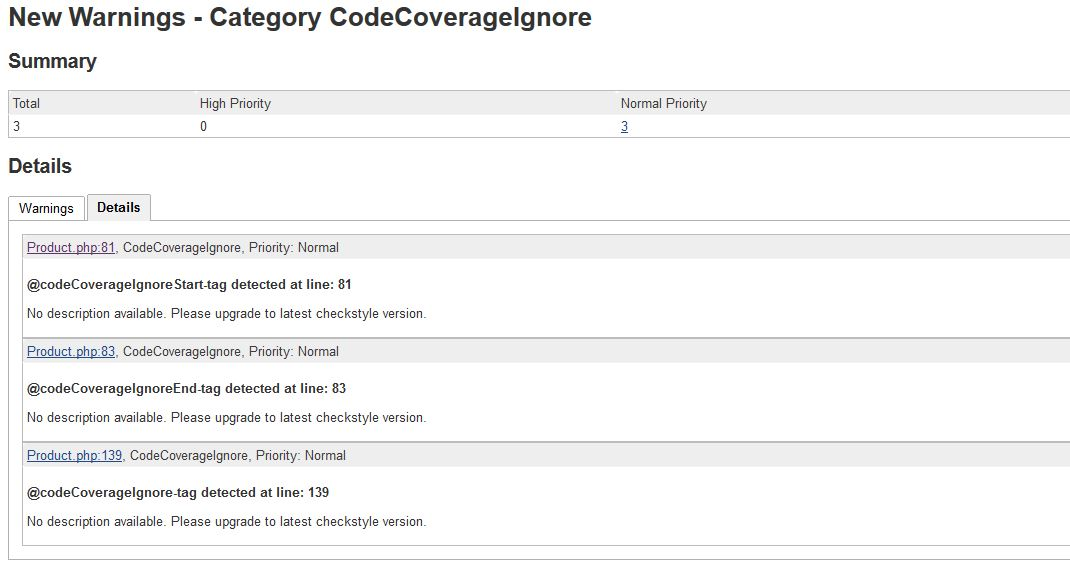
\includegraphics[width=\textwidth]{images/resultSniffer.JPG}
\caption{Ergebnis der CodeSniffer nach Ende eines Build-Jobs \cite{aoe}}
\centering
\end{figure}




\section{Task 11: Webservice für Vertragsverlängerung implementieren}

Der Salespartner hat die Möglichkeit im Congstar Vertriebsportal Verträge eines
Kunden zu verlängern, nachdem der Kunde per mTan authentifiziert wurde. 
Sind die Kundendaten nach der Authentifizierung verfügbar, kann der Salespartner 
sich die Vertragsübersicht des Kunden anzeigen lassen. Durch aktiv gesetzten 
Verlängerungsbutton ist ersichtlich, welcher Vertrag verlängerbar ist.

\begin{figure}[h]
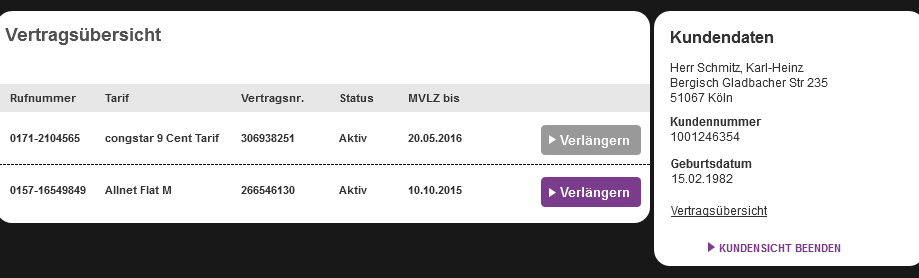
\includegraphics[width=\textwidth]{images/vertragsubersicht.png}
\caption{Vertragsübersicht der Vertragsverlängerung im CPP \cite{congstarv}}
\centering
\end{figure}

Wird der Button gedrückt, löst dieser einen Rest-Call aus, der von eft-rest-api Extension
verarbeitet wird. Diese wiederum spricht die eft-core Extension an, die das backend-seitige Domain-Model abstrahiert. Der Service der eft-core Extension ruft darauf folgend 
die API der eft Extension auf, die letztendlich den zu implementierenden Webservice mit SOAP-Call
auf die AAX$^2$ aufruft. Beim SOAP-Call werden die customerId des Kunden und die contractItemId des zu verlängernden Vertrags mitgegeben. 
Bei erfolgreichem Anfordern der Daten liefert die AAX$^2$ eine ProlongationSuggestionCollection zurück. 
Dabei handelt es um die möglichen Folgeverträge, mit denen 
der Kunde den aktuellen Vertrag verlängern kann. Diese Collection wird bei der Rückgabe ins Frontend sowohl in der eft-core als auch eft-rest-api Extension konvertiert und dann weitergereicht. Anschließend werden die erhaltenen Daten im Frontend gerenderd und der Salespartner landet auf der Bestellübersichtseite (Abbildung \ref{fig:auswahl}), auf der ihm die potenziellen Folgeverträge angezeigt werden. 

\begin{figure}[h]
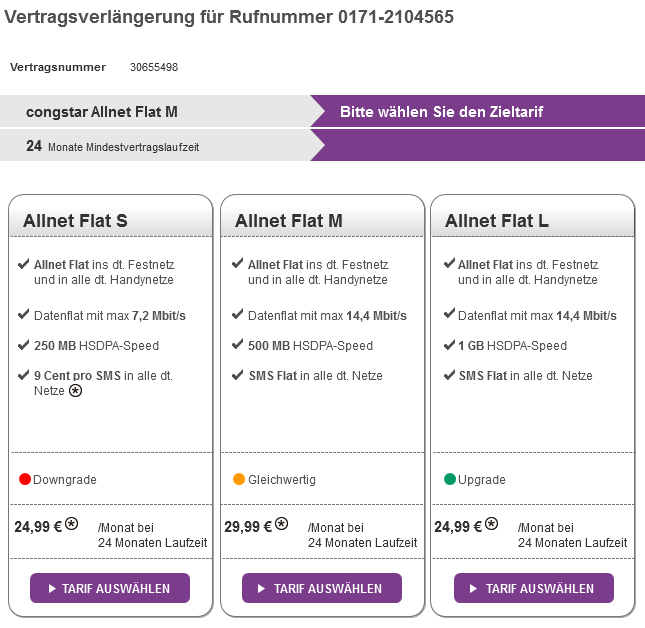
\includegraphics[width=\textwidth]{images/auswahl.png}
\caption{Bestellübersicht der Vertragsverlängerung im CPP \cite{congstarv}}
\centering
\label{fig:auswahl}
\end{figure}


\section{CodeReview}

Nachdem neuer Code entwickelt und durch Unit Tests getestet wurde, erstellt jeder Entwickler ein Code Review Task 
für den eigens geschriebenen Code. Dies geschieht im Congstar Team mit Hilfe von Crucible. Crucible ist ein Tool 
von Atlassien um Code Reviews zu erstellen. Den Code für das Code Review bezieht Crucible dabei direkt
aus den Git- und SVN-Repositories. Durch vorhanden sein der Repository Historie, ist es möglich jeden Commit
mit ins Code Review aufzunehmen, um später gezielt Änderungen betrachten zu können. Der in Crucible sichtbare Code
kann dort direkt mit Kommentaren und Verbesserungsvorschlägen versehen werden.
Gegen Ende meines Praktikums vielen auch solche Tasks in meinen Aufgabenbereich.


\section{Behobene Issues} \label{sec:issues}

\subsection{Issue 01: Optionsmanagement CSC - Optimierung der Anzeige für gebuchte Optionen}

Congstar bietet seinen Kunden im CSC seines Webshops die Möglichkeit jederzeit neue Optionen dazu zu buchen oder umzubuchen.
Dabei gibt es Optionen in drei Kategorien: Optionen für SMS, für mobiles Internet und für Telefonie.
Für ein Tarif Produkt kann jedoch nur eine Option pro Optionskategorie ausgewählt werden.

Thema dieses Issues war, dass auch bei drei gebuchten Optionen aus jeder Kategorie noch der Bereich anzeigt wird,
indem die zu buchbaren Optionen stehen sollten. Wenn jedoch aus jeder Kategorie bereits eine Option gebucht ist,
soll es nicht möglich sein weitere Optionen zu buchen. Wie in Abbildung \ref{fig:optZuBuch} zu sehen, wurde der 
Bereich für die zu-buchbaren Optionen weiterhin angezeigt, auch wenn keine Optionen mehr vorhanden waren.

Was fehlte, war lediglich eine Überprüfung, ob in jeder Kategorie bereits eine Option ausgewählt ist, um das Template
in diesem Fall ohne den Bereich der zu-buchbaren Optionen anzuzeigen.

\begin{figure}[h] 
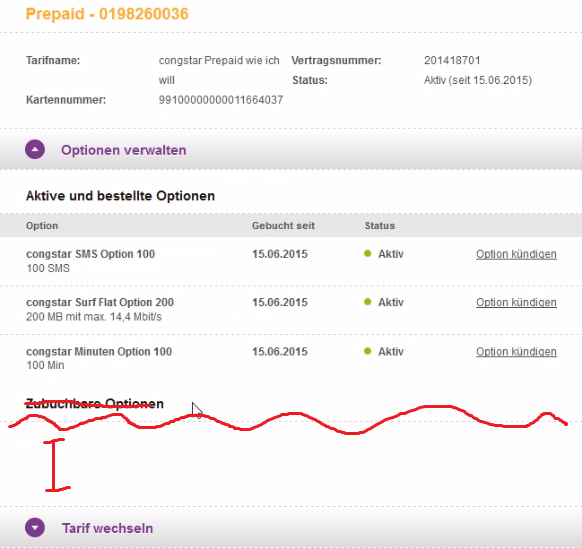
\includegraphics[width=\textwidth]{images/optionenzubuchun.png}
\caption{Übersicht der Optionen die im CSC verwaltet werden können \cite{congstarv}}
\label{fig:optZuBuch}
\centering 
\end{figure}


\subsection{Issue 02: Abstände auf der MeineProdukte-Seite im CSC auf den Inhalt anpassen} \label{sec:issue02}

Das Problem bei diesem Issue bestand darin, dass der Style des Templates an einer bestimmten Stelle für den Text
der Tarifnamen fest definiert war und so bei langen Tarifnamen der Text unschön umgebrochen ist.
Hier mussten lediglich Änderungen im SCSS vorgenommen werden, wodurch ich den Umgang mit SASS und compass
kennengelernt habe.


\subsection{Issue 03: Abstände auf der MeineProdukte-Seite (Übersicht) im CSC auf den Inhalt anpassen} 

Ähnlich wie in Issue \ref{sec:issue02} waren hier Änderungen im SCSS für ein Template notwenig, sodass
der Tarifname bei der Produktübersichtsseite nicht mehr umbricht (Abbildung \ref{fig:xxx}).

\begin{figure}[h] 
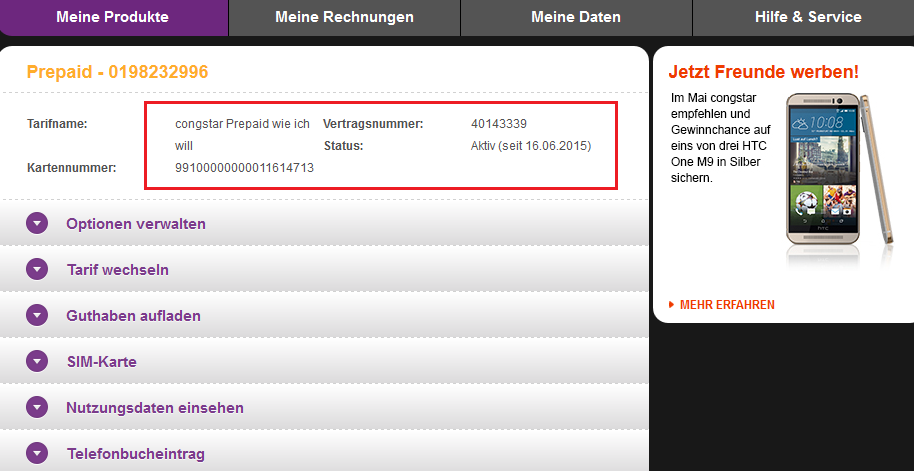
\includegraphics[width=\textwidth]{images/csc.PNG}
\caption{Übersicht der "Meine Produkte"-Seite im CSC \cite{congstarcsc}}
\centering
\label{fig:xxx}
\end{figure}


\subsection{Issue 04: Anpassung des Hinweistexts zur Triple-SIM} 

Nach Auswahl eines Tarifs und Auswahl eines Handys für diesen Tarif, gelangt man im nächsten Schritt 
auf die Auswahlseite für die SIM-Karte. In der Vergangenheit bestand die Möglichkeit abhängig vom
SIM-Kartentyp des Handys zwischen einer Nano, Hybrid oder Triple SIM-Karte zu wählen.

Inzwischen ist es jedoch so, dass unabhängig vom Gerät und benötigter SIM-Karte nur noch die Triple SIM-Karte
ausgeliefert wird. Diese bietet für alle Gerätetypen, die passende SIM-Karte. 
Wie in Abbildung \ref{fig:triple} treten bei der Anzeige der verschiedenen Informationen noch Fehler auf.
\begin{figure}[h] 
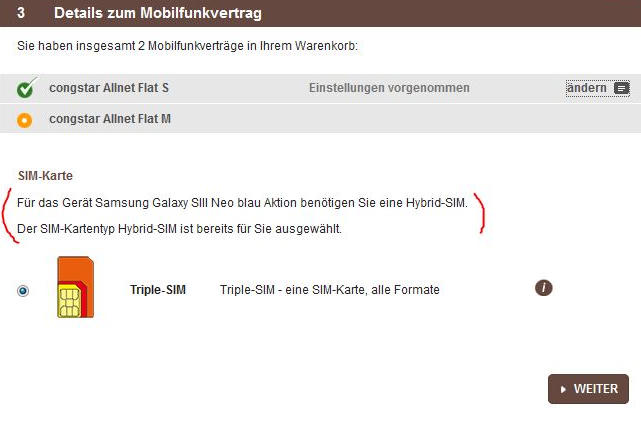
\includegraphics[width=\textwidth]{images/triple.PNG}
\caption{Vorausgewählte Triple SIM-Karte \cite{congstar}}
\label{fig:triple}
\centering
\end{figure}
Bei den beiden Sätzen: 'Für das Gerät Samsung Galaxy SIII Neo blau Aktion benötigen Sie eine Hybrid-SIM. Der SIM-Kartentyp Hybrid-SIM ist bereits für Sie ausgewählt.', wird der Name der SIM-Karte dynamisch aus den Handyobjekt geladen und ins Template gerendert, während die Auswahl 'Triple -SIM - eine SIM-Karte, alle Formate' hart gecoded wurde. 

Der Code wurde deshalb so geändert, dass für die Beschreibung für die bereits ausgewählte SIM-Karte ebenfalls die Triple-SIM ausgegeben wird.


\subsection{Issue 05: Vertragsübersicht bei Vertragsverlängerung: Tarife zeigen teilweise keine Telefonnummer an}

Möchte man die verschiedenen Verträge eines Kunden im CPP anzeigen, wird der Webservice getCustomerFull()
\begin{lstlisting}
public function getCustomerFull($customerId)
\end{lstlisting}
aufgerufen, der ein Kunden-Objekt zurückliefert. Diese Kundenobjekt beinhaltet das Contract-Objekt 
und das wiederum mehrere ContractItem-Objekte, die letztendlich die Vertragsinformationen 
zu Produkten und Optionen beinhalten.
Das Ergebnis der AAX$^2$ wird in der eft Extension zu den eben erwähnten Objekten verarbeitet. 
Das ContractItem besitzt mehrere Arten von Telefonnummern, die sich unterscheiden lassen.
Schließt ein Neukunde einen Vertrag mit einer neuen Nummer bei Congstar ab, so wird die Nummer in der Standardliste
für Telefonnummern abgelegt und kann dort abgefragt werden. Wechselt ein Kunde jedoch von einem anderen Anbieter
zu Congstar und möchte seine Rufnummer mitnehmen, so wird diese Nummer als ported gekennzeichnet und taucht nicht 
in der Standardliste auf. Dritter Fall tritt auf wenn ein Vertrag bereits aktiv ist, die Rufnummer jedoch erst bestellt
und somit noch keine Rufnummer vorhanden ist.

Das Problem, dass bei der Vertragsübersicht bei manchen Verträgen keine Nummer angezeigt wurde, lag daran, dass 
lediglich die Standardliste angefragt wurde. Genauer erklärt, passierte das bei der Konvertierung von einem eft ContractItem-Objekt
zu einem eft-core ContractItem-Objekt.

Das Problem wurde behoben indem bei der Konvertierung beide Listen angefragt werden um zu prüfen ob überhaupt eine Nummer vorhanden ist. Der lediglich der entweder oder Fall auftreten kann, wird die vorhandene Nummer ausgewählt. Wenn jedoch keine Nummer vorhanden ist wird im Frontend ein Hinweistext anstelle der Nummer ausgegeben.


\newpage

\listoffigures % Liste der Abbildungen
\bibliographystyle{plain}
\bibliography{ausarb}

% zum Beispiel mit bibtopic kann man die Quellen sauber trennen
%\begin{btSect}{ausarb}
%\section*{Literaturverzeichnis}
%\bibliography{mybib}{}
%\bibliographystyle{plain}
%\btPrintCited
%\end{btSect}
\begin{btSect}{online}
\section*{Online-Quellen}
\btPrintCited
\end{btSect}
% dann mit "bibtex ausarb1" und "bibtex ausarb2" arbeiten
% Wir verwenden ausarb<i> weil die Dokumenten-Datei ausarb.tex ist


\end{document}
